\chapter{Diseño e implementación}

En este capítulo se documenta el diseño e implementación que se ha realizado para dar lugar a la aplicación final. Como bien se explica en el capítulo dedicado a la arquitectura, se ha seguido una división por subsistemas por lo que la mejor aproximación para separar ahora los múltiples diagramas de clases es hacerlo por paquetes, asociados cada uno de ellos a un subsistema. Además se generarán una serie de paquetes que contienen una serie de funcionalidades adicionales utilizadas por los otros.

\bigskip

Se empezará por la documentación asociada a los paquetes relacionados con el motor del videojuego en sí mismo para luego seguir con el subsistema de la lógica de la aplicación que contendrá la implementación del agente. Luego se muestran los diagramas de interacción que relacionan las clases antes definidas con los casos de uso en los que participan. Finalmente se mostrará como se llegó al diseño de la interfaz gráfica de la aplicación.

\section{Diagramas de clases}


\begin{figure}
	\centerline{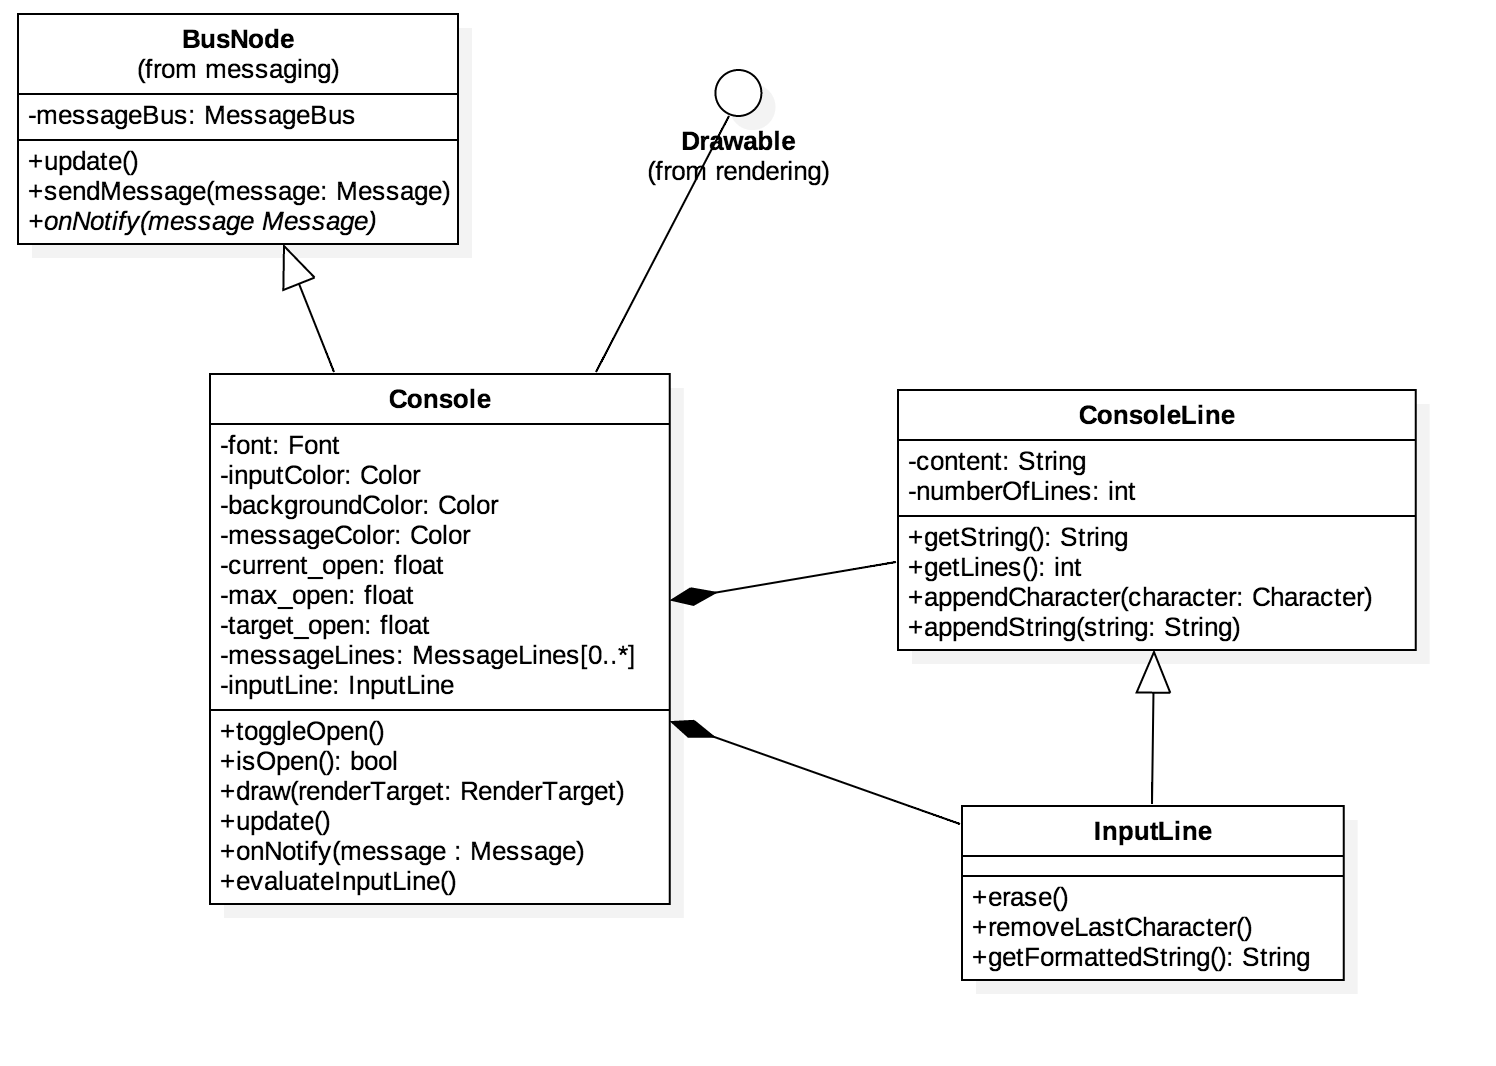
\includegraphics[width=15cm]{otros/UML/png/alld/png/console__diagramaDeClases_console_3.png}}
	\caption{Diagrama de clases del subsistema de consola}
	\label{class:console}
\end{figure}

\begin{figure}
	\centerline{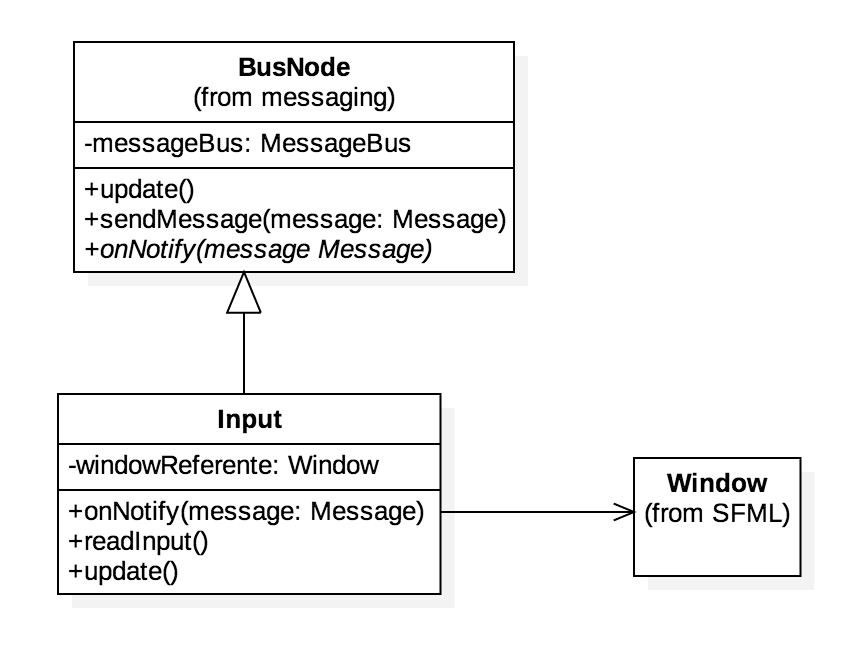
\includegraphics[width=12cm]{otros/UML/png/alld/png/input__diagramaDeClases_input_8.png}}
	\caption{Diagrama de clases del subsistema de entrada}
	\label{class:input}
\end{figure}

\begin{figure}
	\centerline{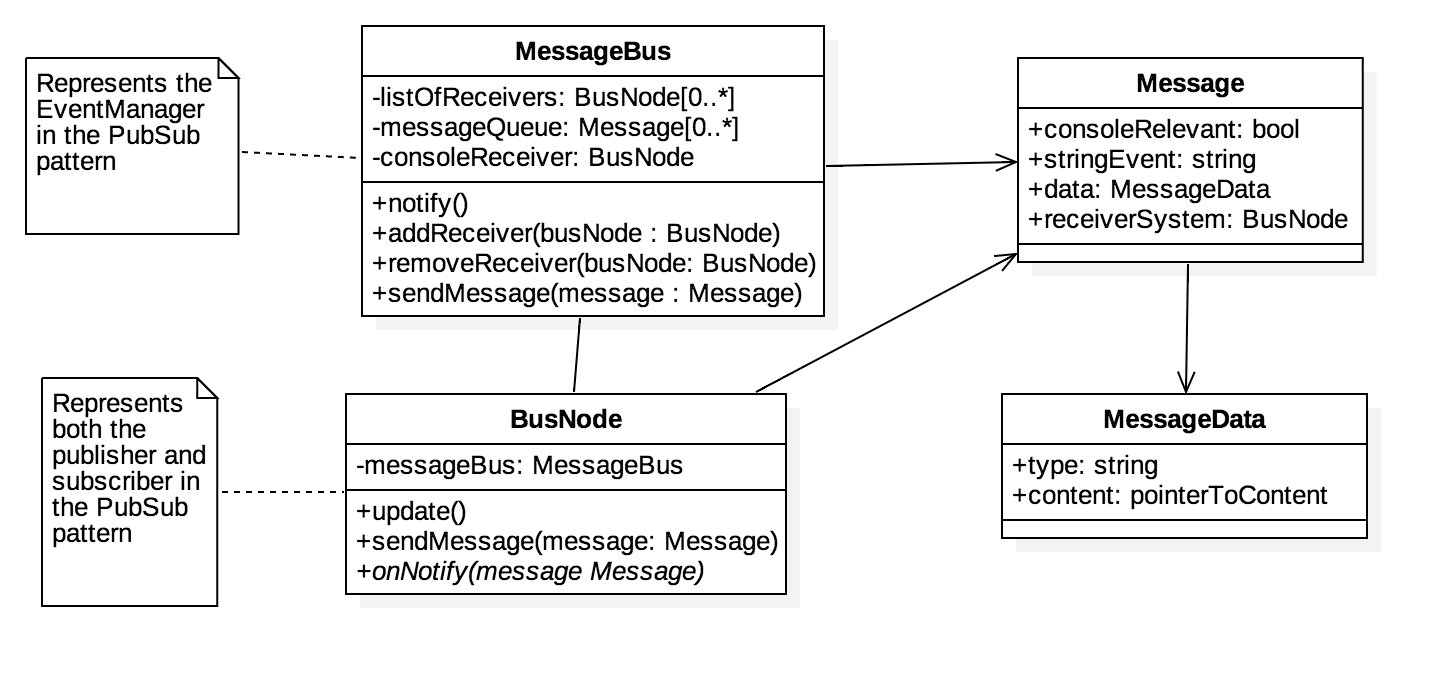
\includegraphics[width=15cm]{otros/UML/png/alld/png/messaging__diagramaDeClases_messaging_11.png}}
	\caption{Diagrama de clases del bus de mensajes}
	\label{class:messageBus}
\end{figure}

\begin{figure}
	\centerline{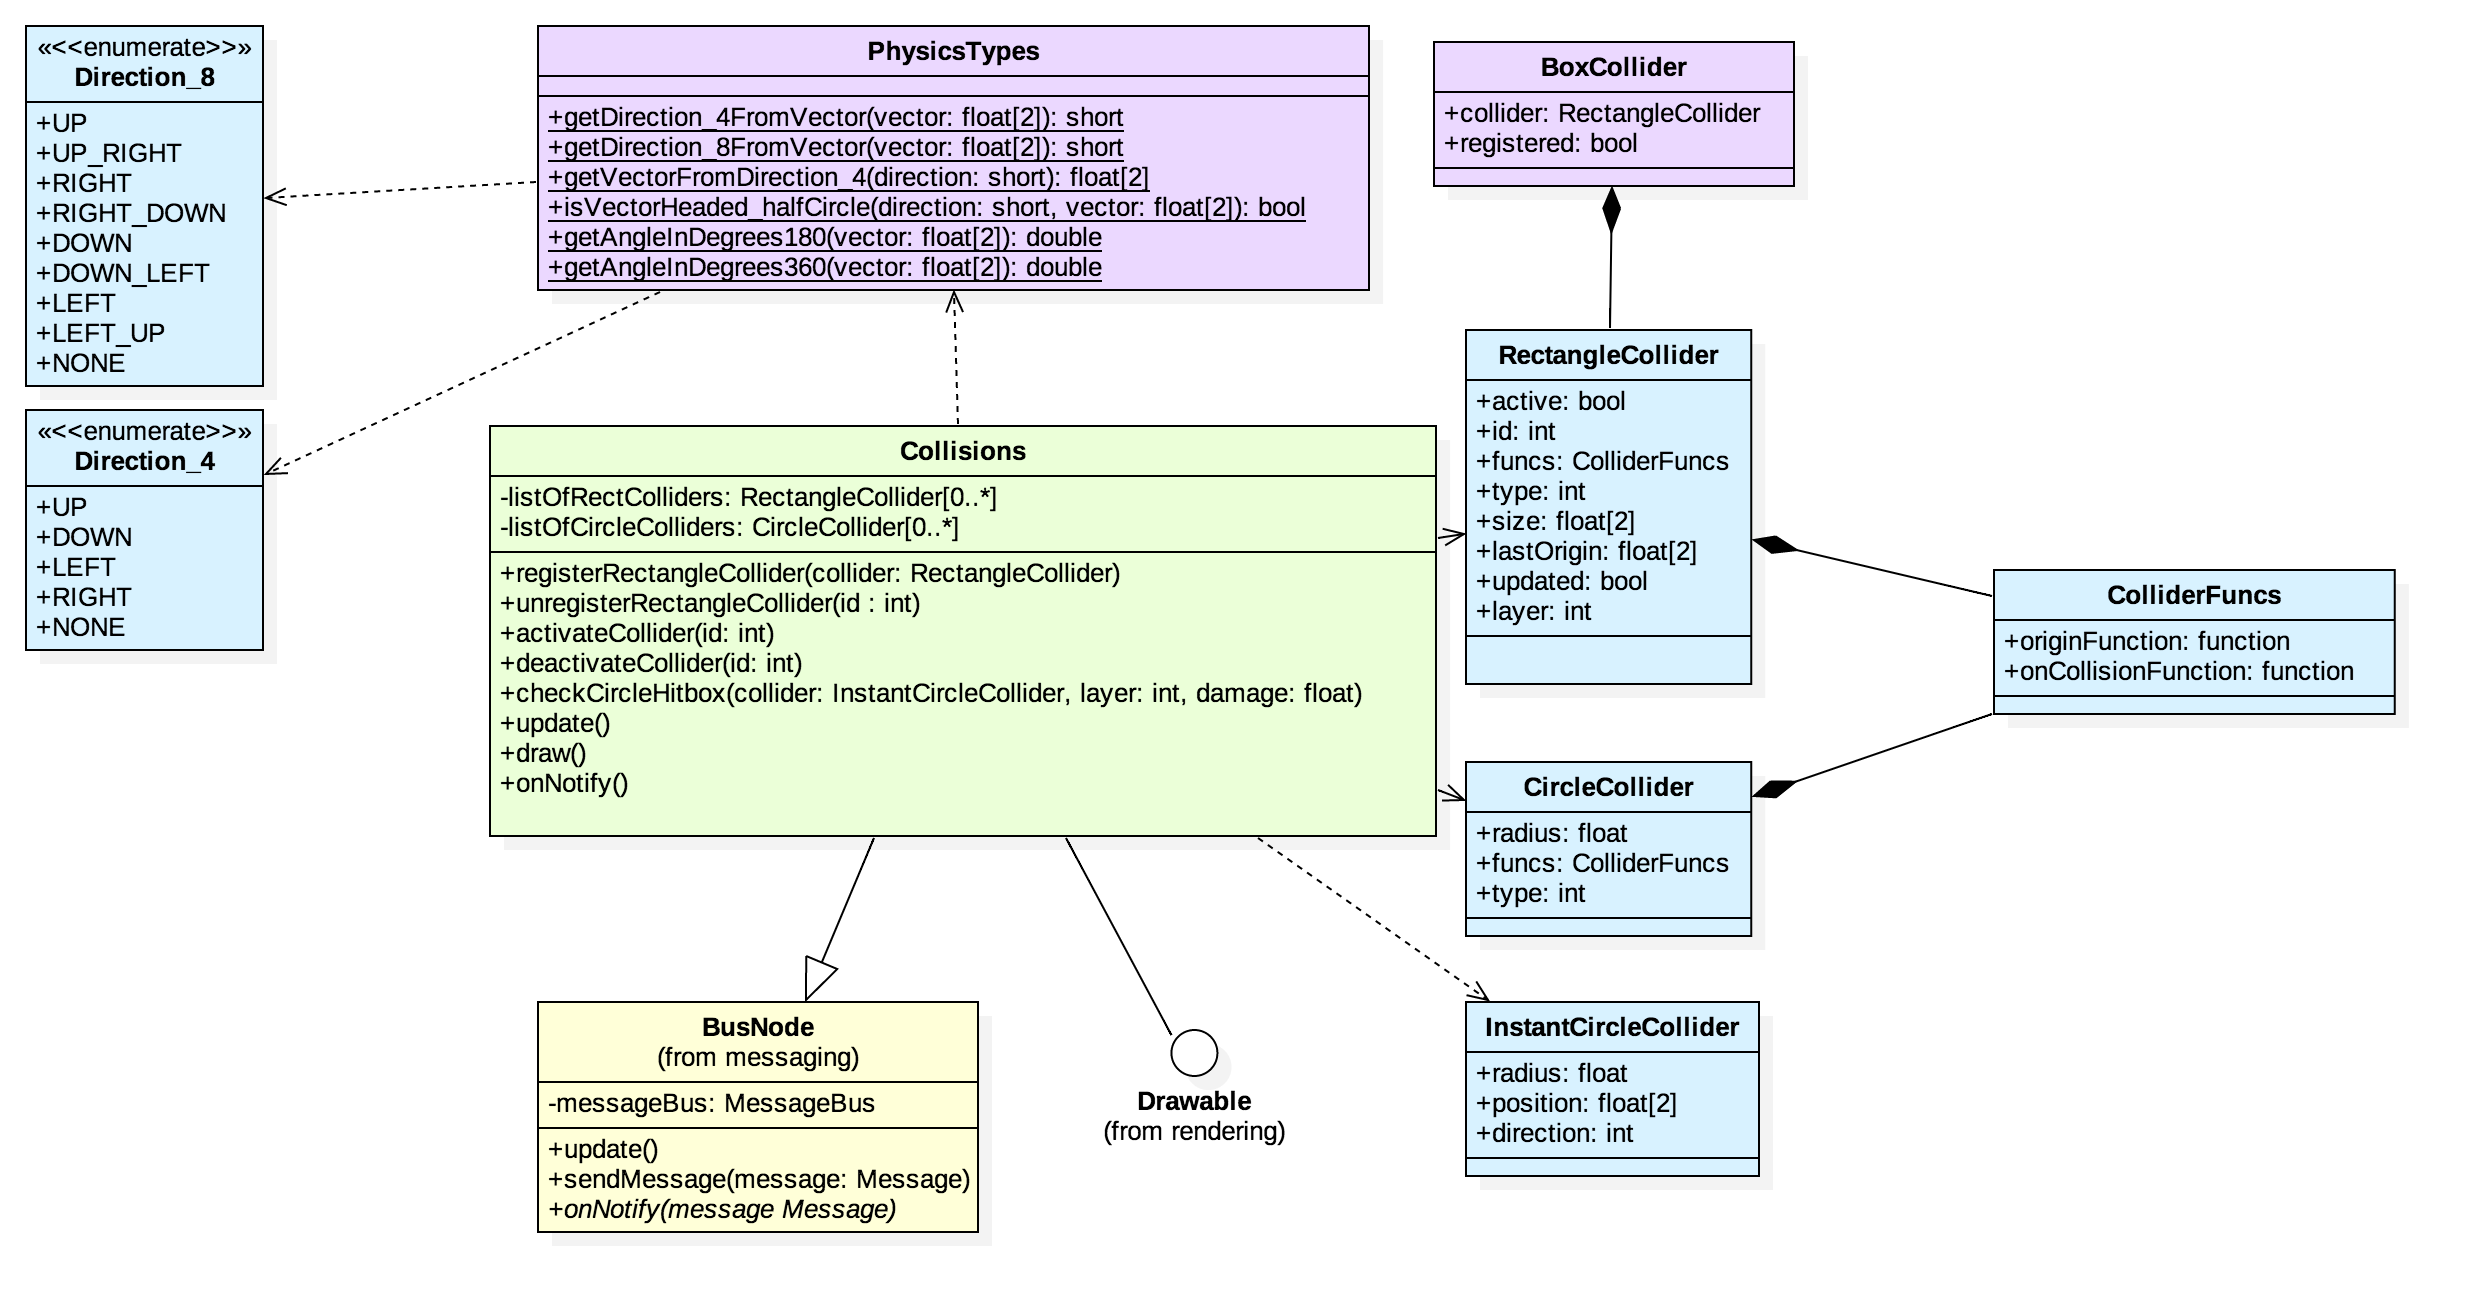
\includegraphics[width=18cm]{otros/UML/png/alld/png/physics__diagramaDeClases_physics_2.png}}
	\caption{Diagrama de clases del subsistema de físicas}
	\label{class:collisions}
\end{figure}

\begin{figure}
	\centerline{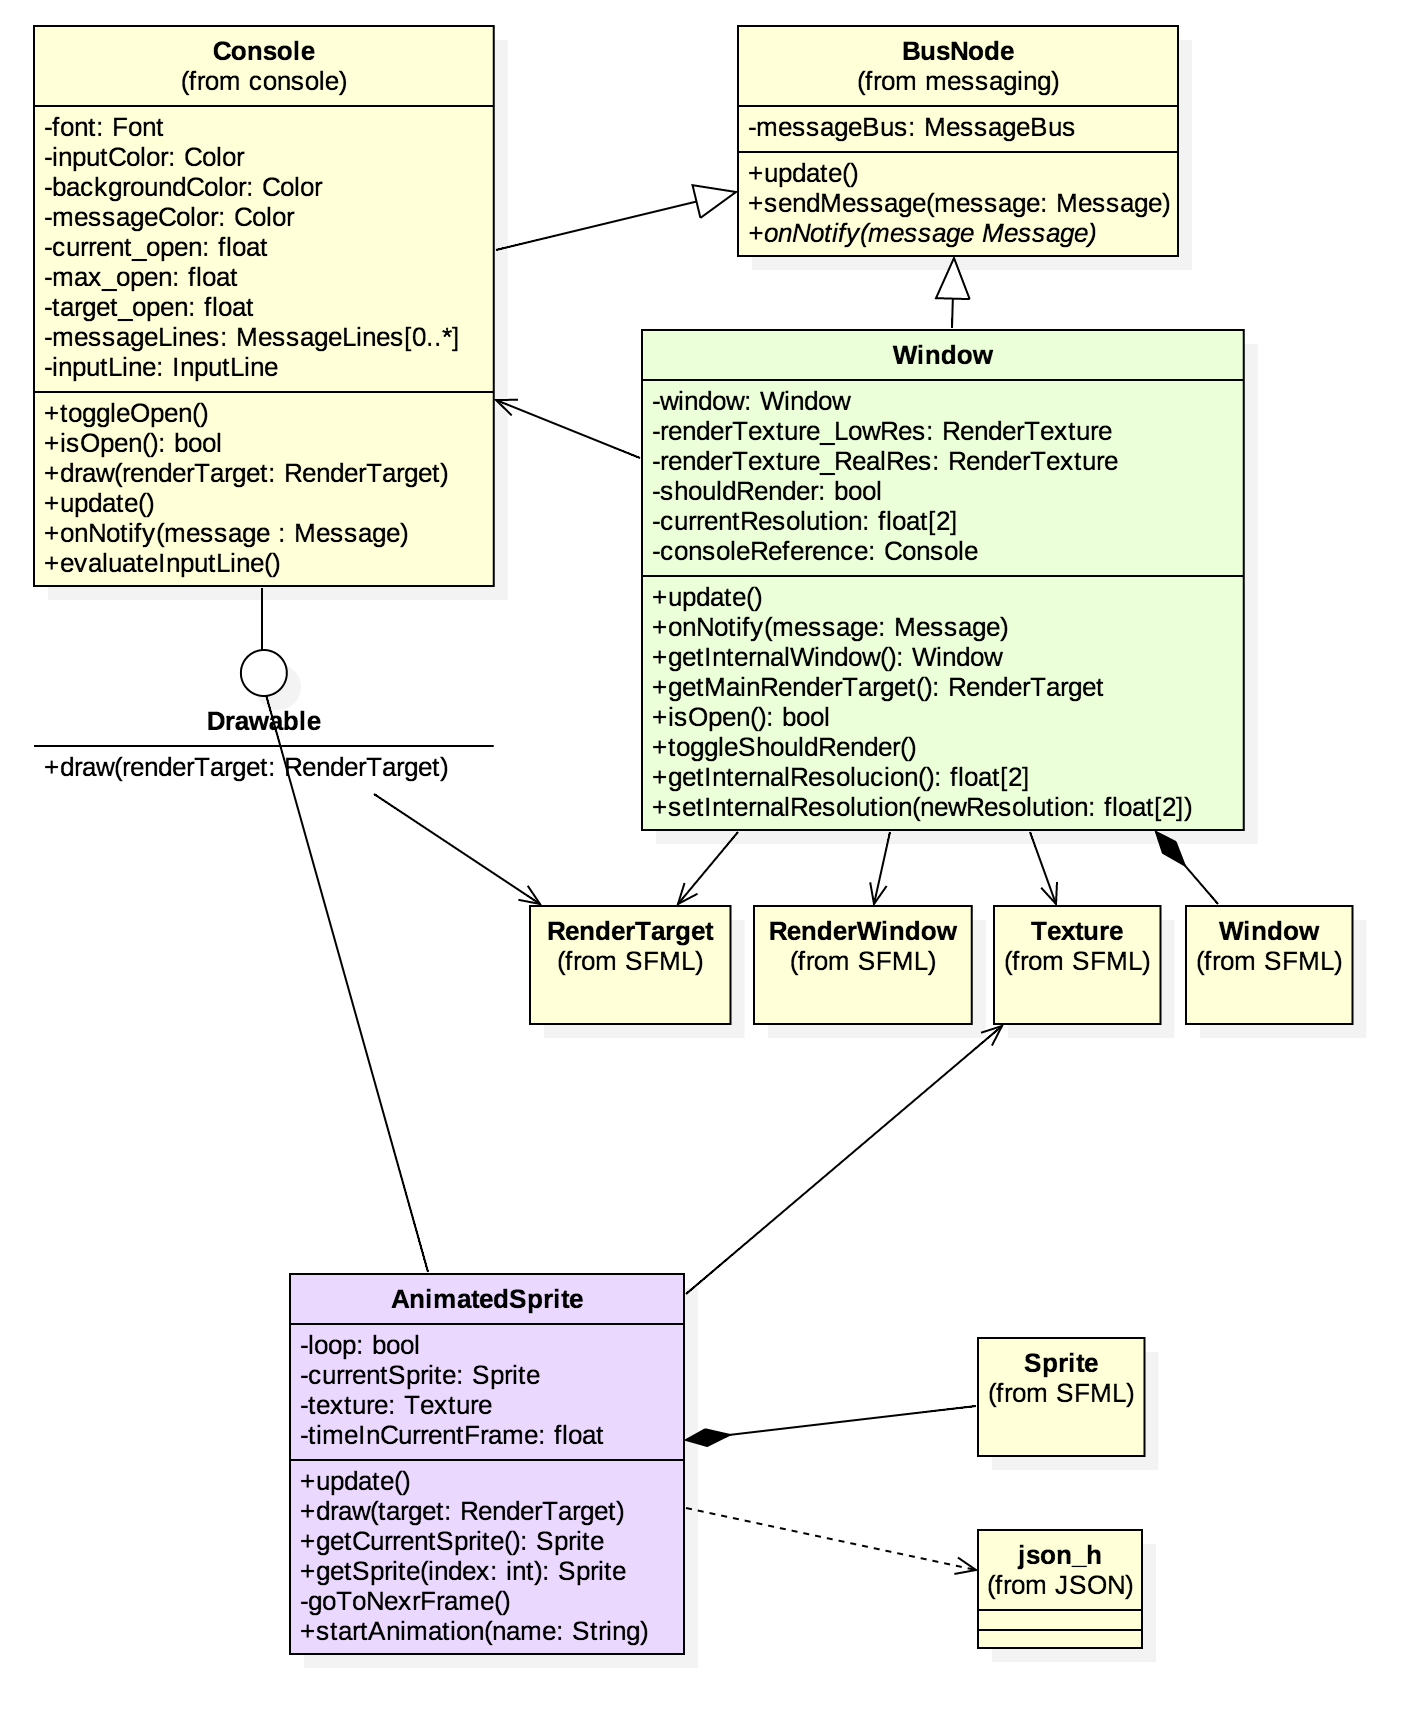
\includegraphics[width=15cm]{otros/UML/png/alld/png/rendering__diagramaDeClases_rendering_9.png}}
	\caption{Diagrama de clases del subsistema de renderizado}
	\label{class:rendering}
\end{figure}


\begin{figure}
	\centerline{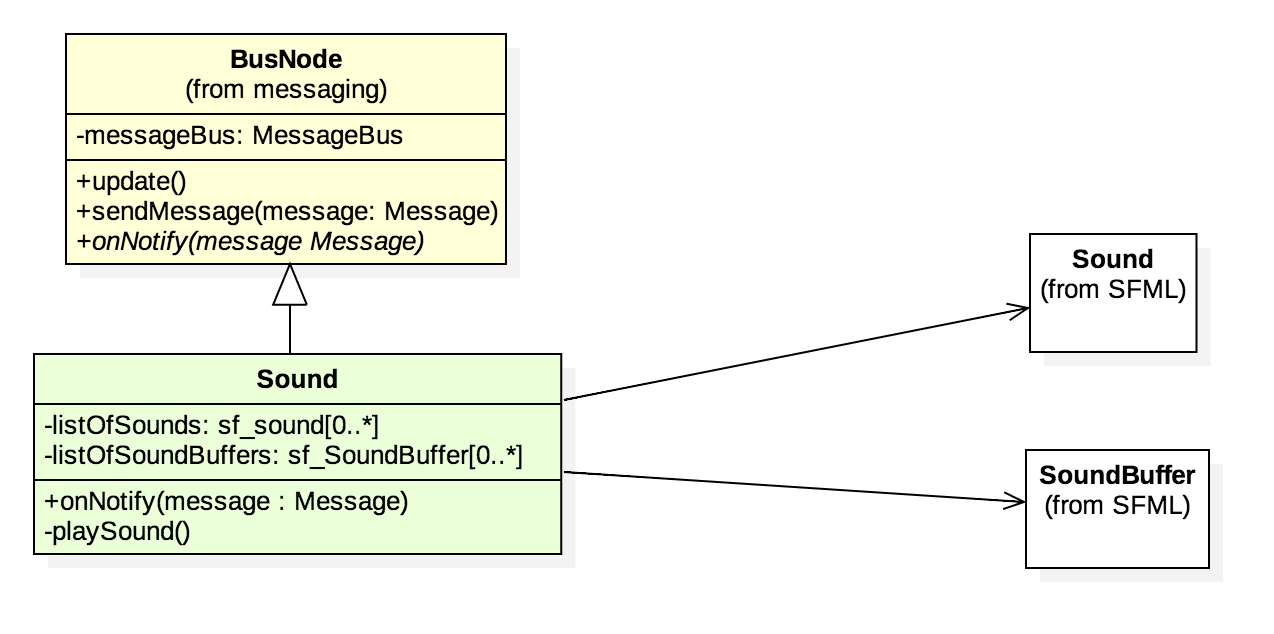
\includegraphics[width=15cm]{otros/UML/png/alld/png/sound__diagramaDeClases_sound_1.png}}
	\caption{Diagrama de clases del subsistema de sonido}
	\label{class:sound}
\end{figure}

\begin{figure}
	\centerline{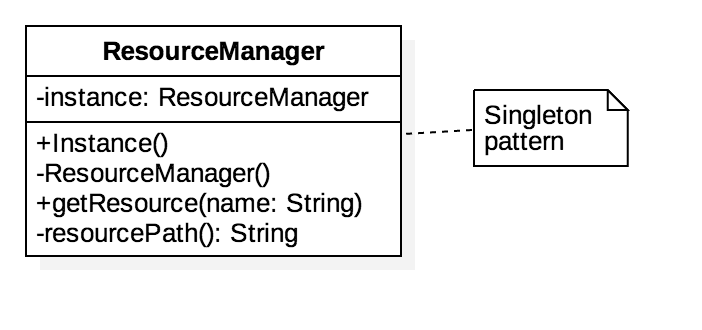
\includegraphics[width=8cm]{otros/UML/png/alld/png/resources__diagramaDeClases_resources_0.png}}
	\caption{Diagrama de clases del paquete de recursos}
	\label{class:resources}
\end{figure}

\begin{figure}
	\centerline{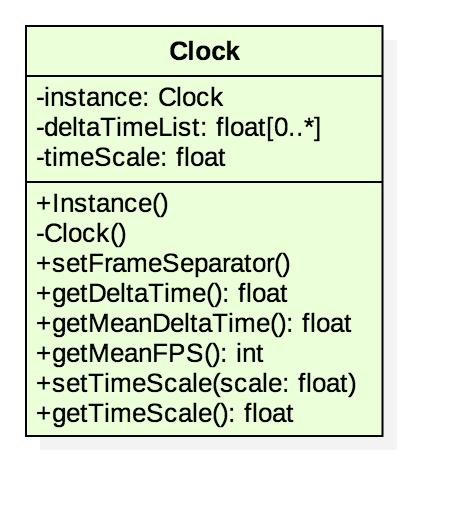
\includegraphics[width=5cm]{otros/UML/png/alld/png/utils__diagramaDeClases_utils_10.png}}
	\caption{Diagrama de clases del paquete de útiles}
	\label{class:utils}
\end{figure}

\begin{figure}
	\centerline{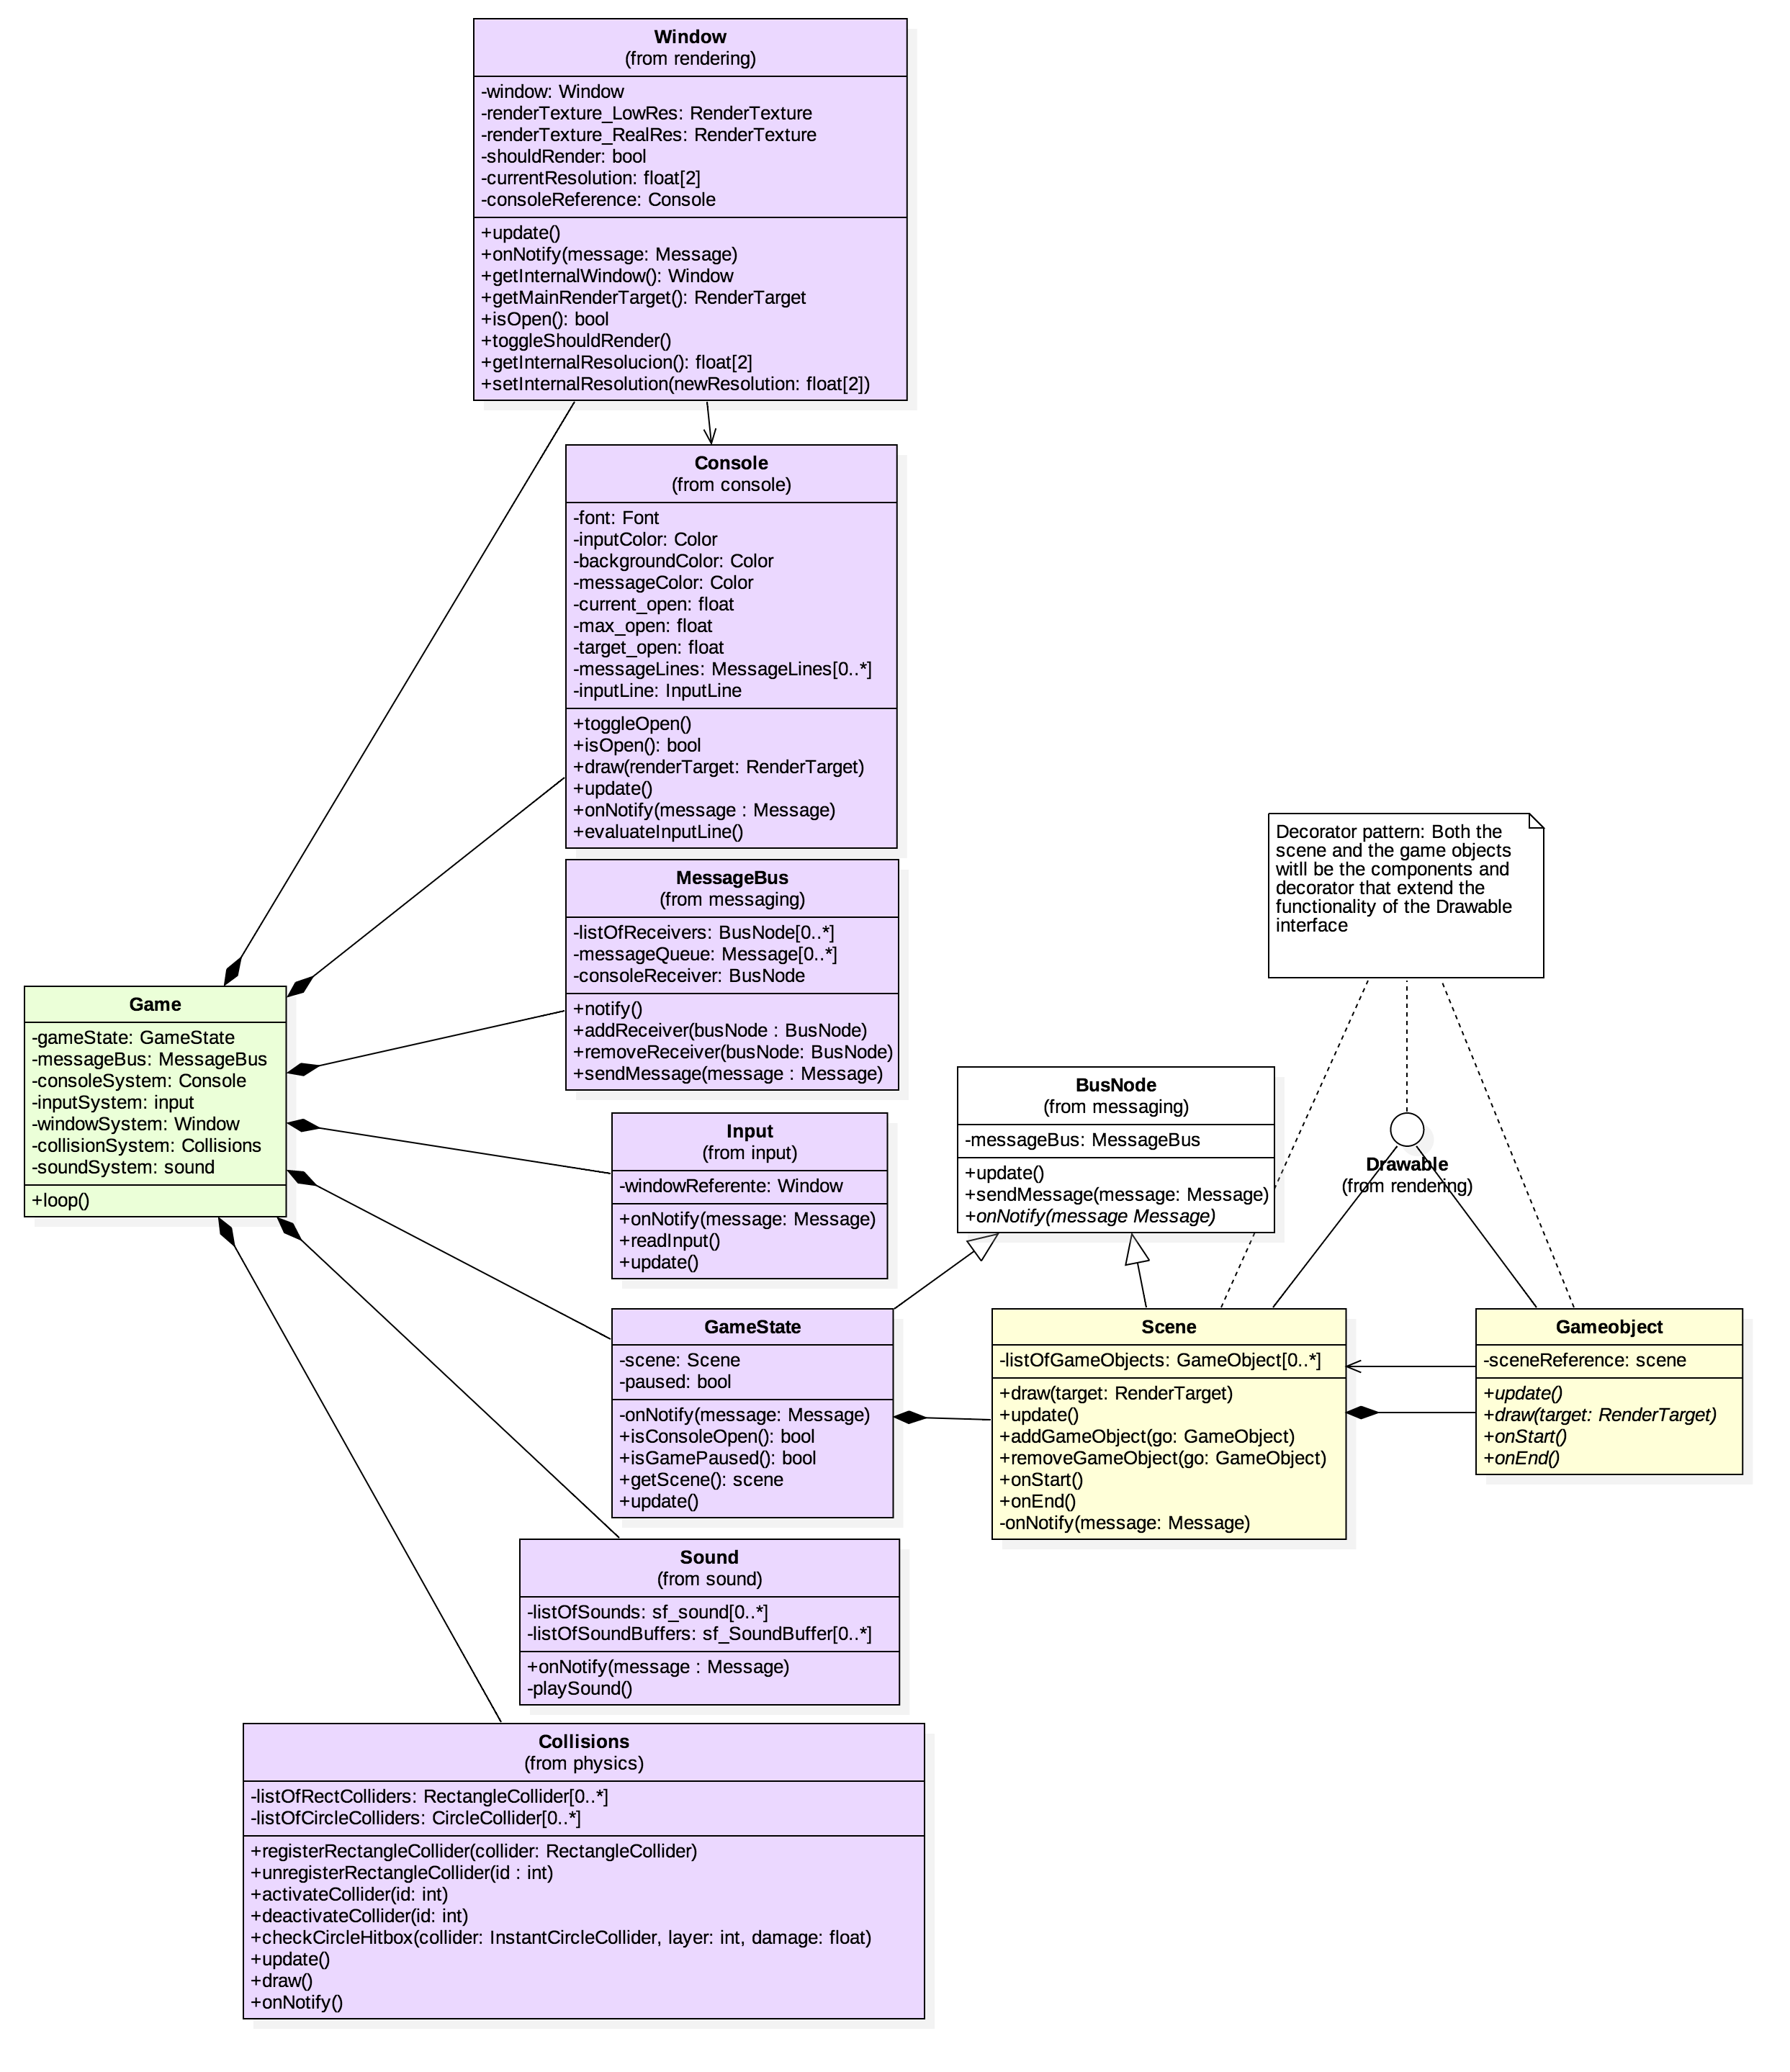
\includegraphics[width=18cm]{otros/UML/png/alld/png/gamelogic__diagramaDeClases_gamelogic_7.png}}
	\caption{Diagrama de clases de la lógica del juego}
	\label{class:gamelogic}
\end{figure}

\begin{figure}
	\centerline{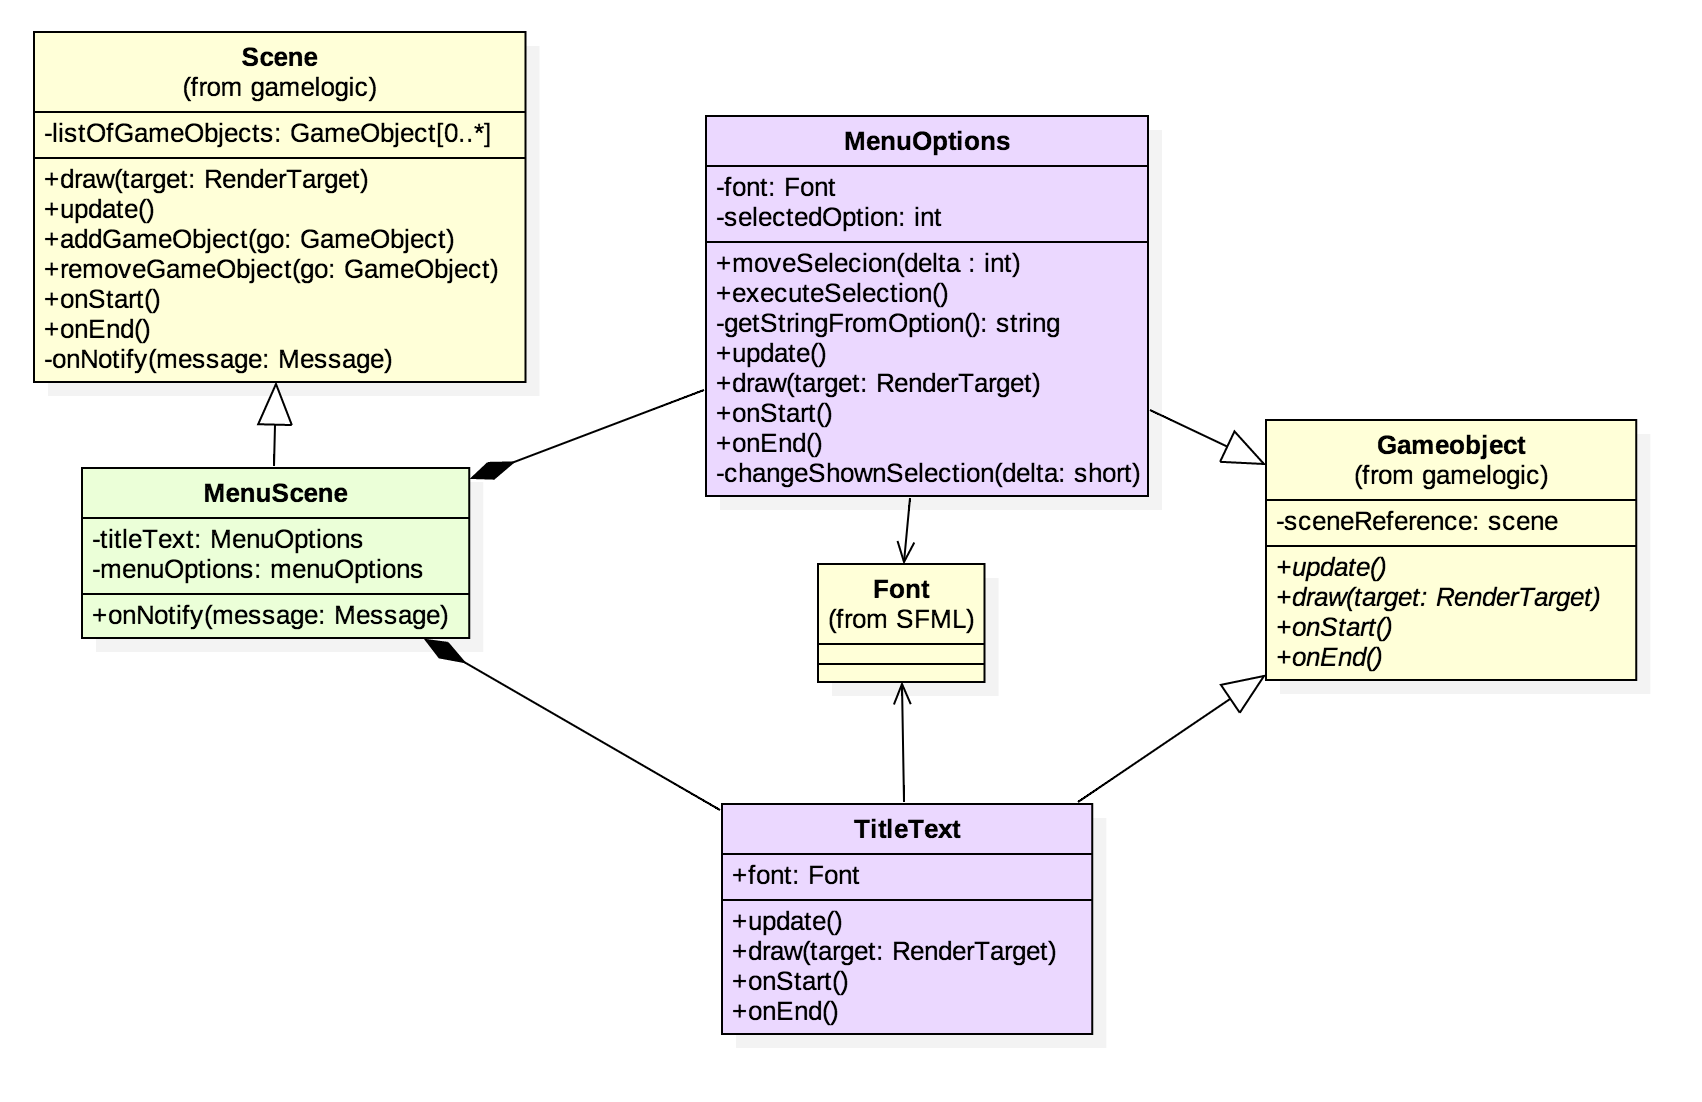
\includegraphics[width=15cm]{otros/UML/png/alld/png/gamelogic__menu__diagramaDeClases_scene_menu_6.png}}
	\caption{Diagrama de clases de la escena del menú}
	\label{class:scene}
\end{figure}

\begin{figure}
	\begin{adjustwidth}{+3cm}{}
	\caption{Diagrama de clases de la escena de juego}
	\centerline{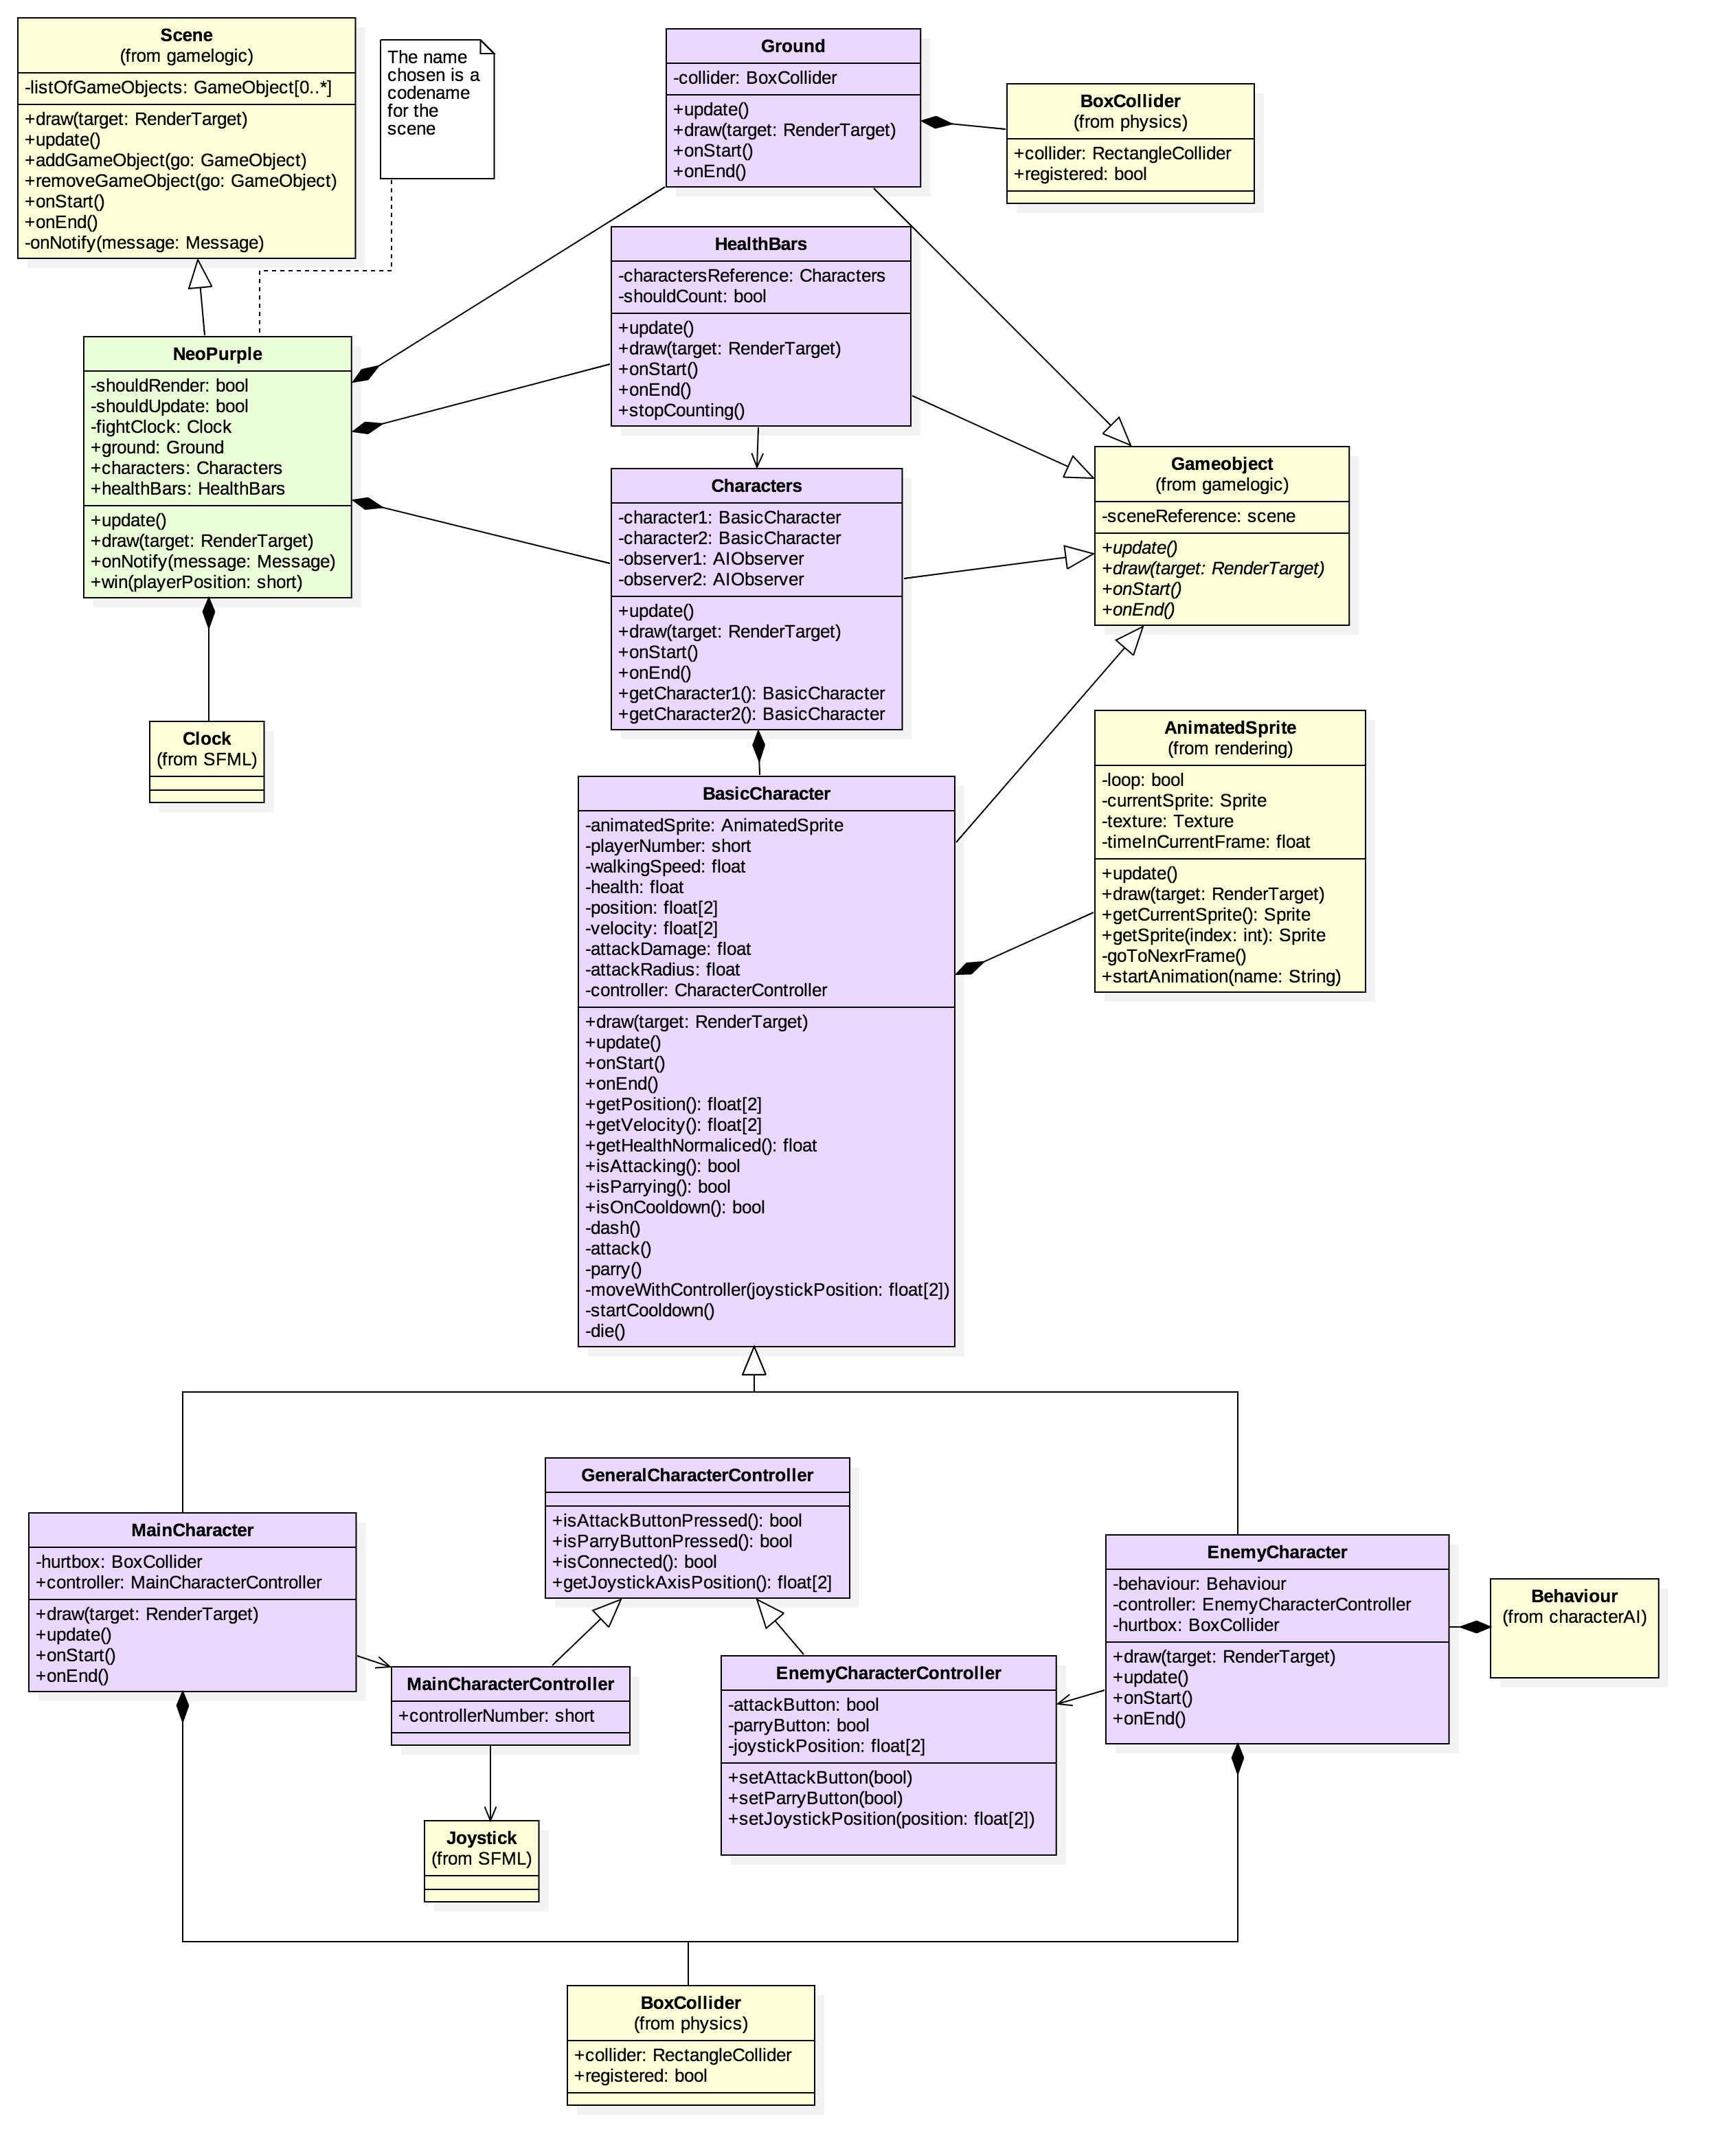
\includegraphics[width=20cm]{otros/UML/png/alld/png/gamelogic__gameplay__diagramaDeClases_scene_gameplay_4.png}}
	\label{class:gameplay}
\end{adjustwidth}
\end{figure}

\clearpage
\begin{landscape}
\begin{figure}
	\begin{adjustwidth}{-3cm}{}
		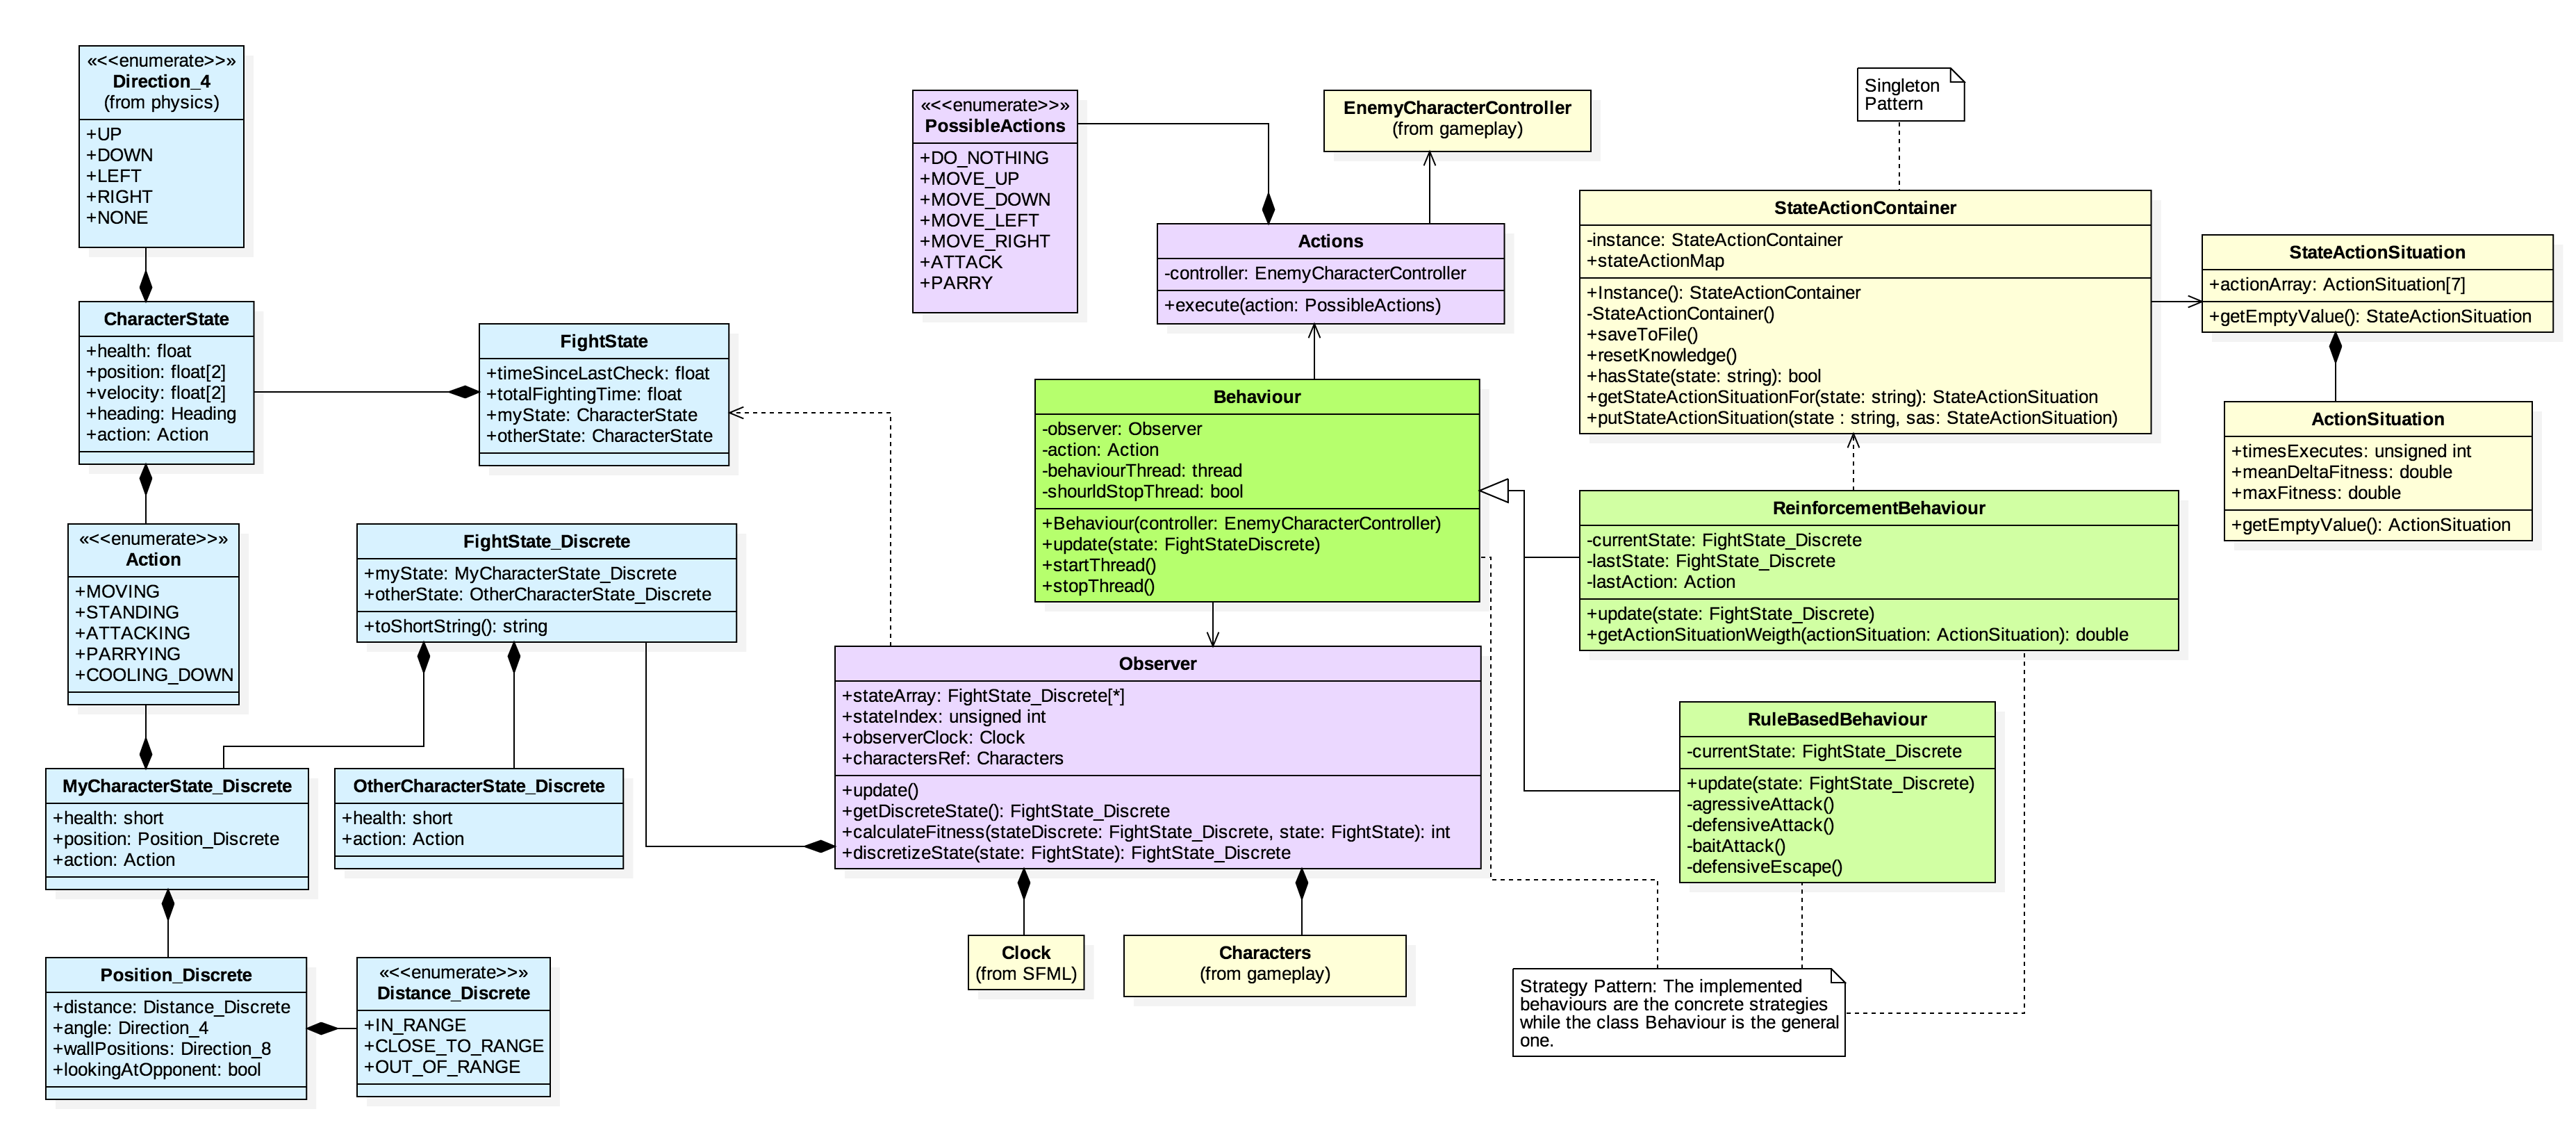
\includegraphics[width=24cm]{otros/UML/png/alld/png/gamelogic__gameplay__characterAI__diagramaDeClases_IA_5.png}
		\caption{Diagrama de clases del comportamiento del agente}
		\label{class:agent}
	\end{adjustwidth}
\end{figure}
\end{landscape}
\clearpage


\section{Diagramas de secuencia}

\begin{figure}
	\centerline{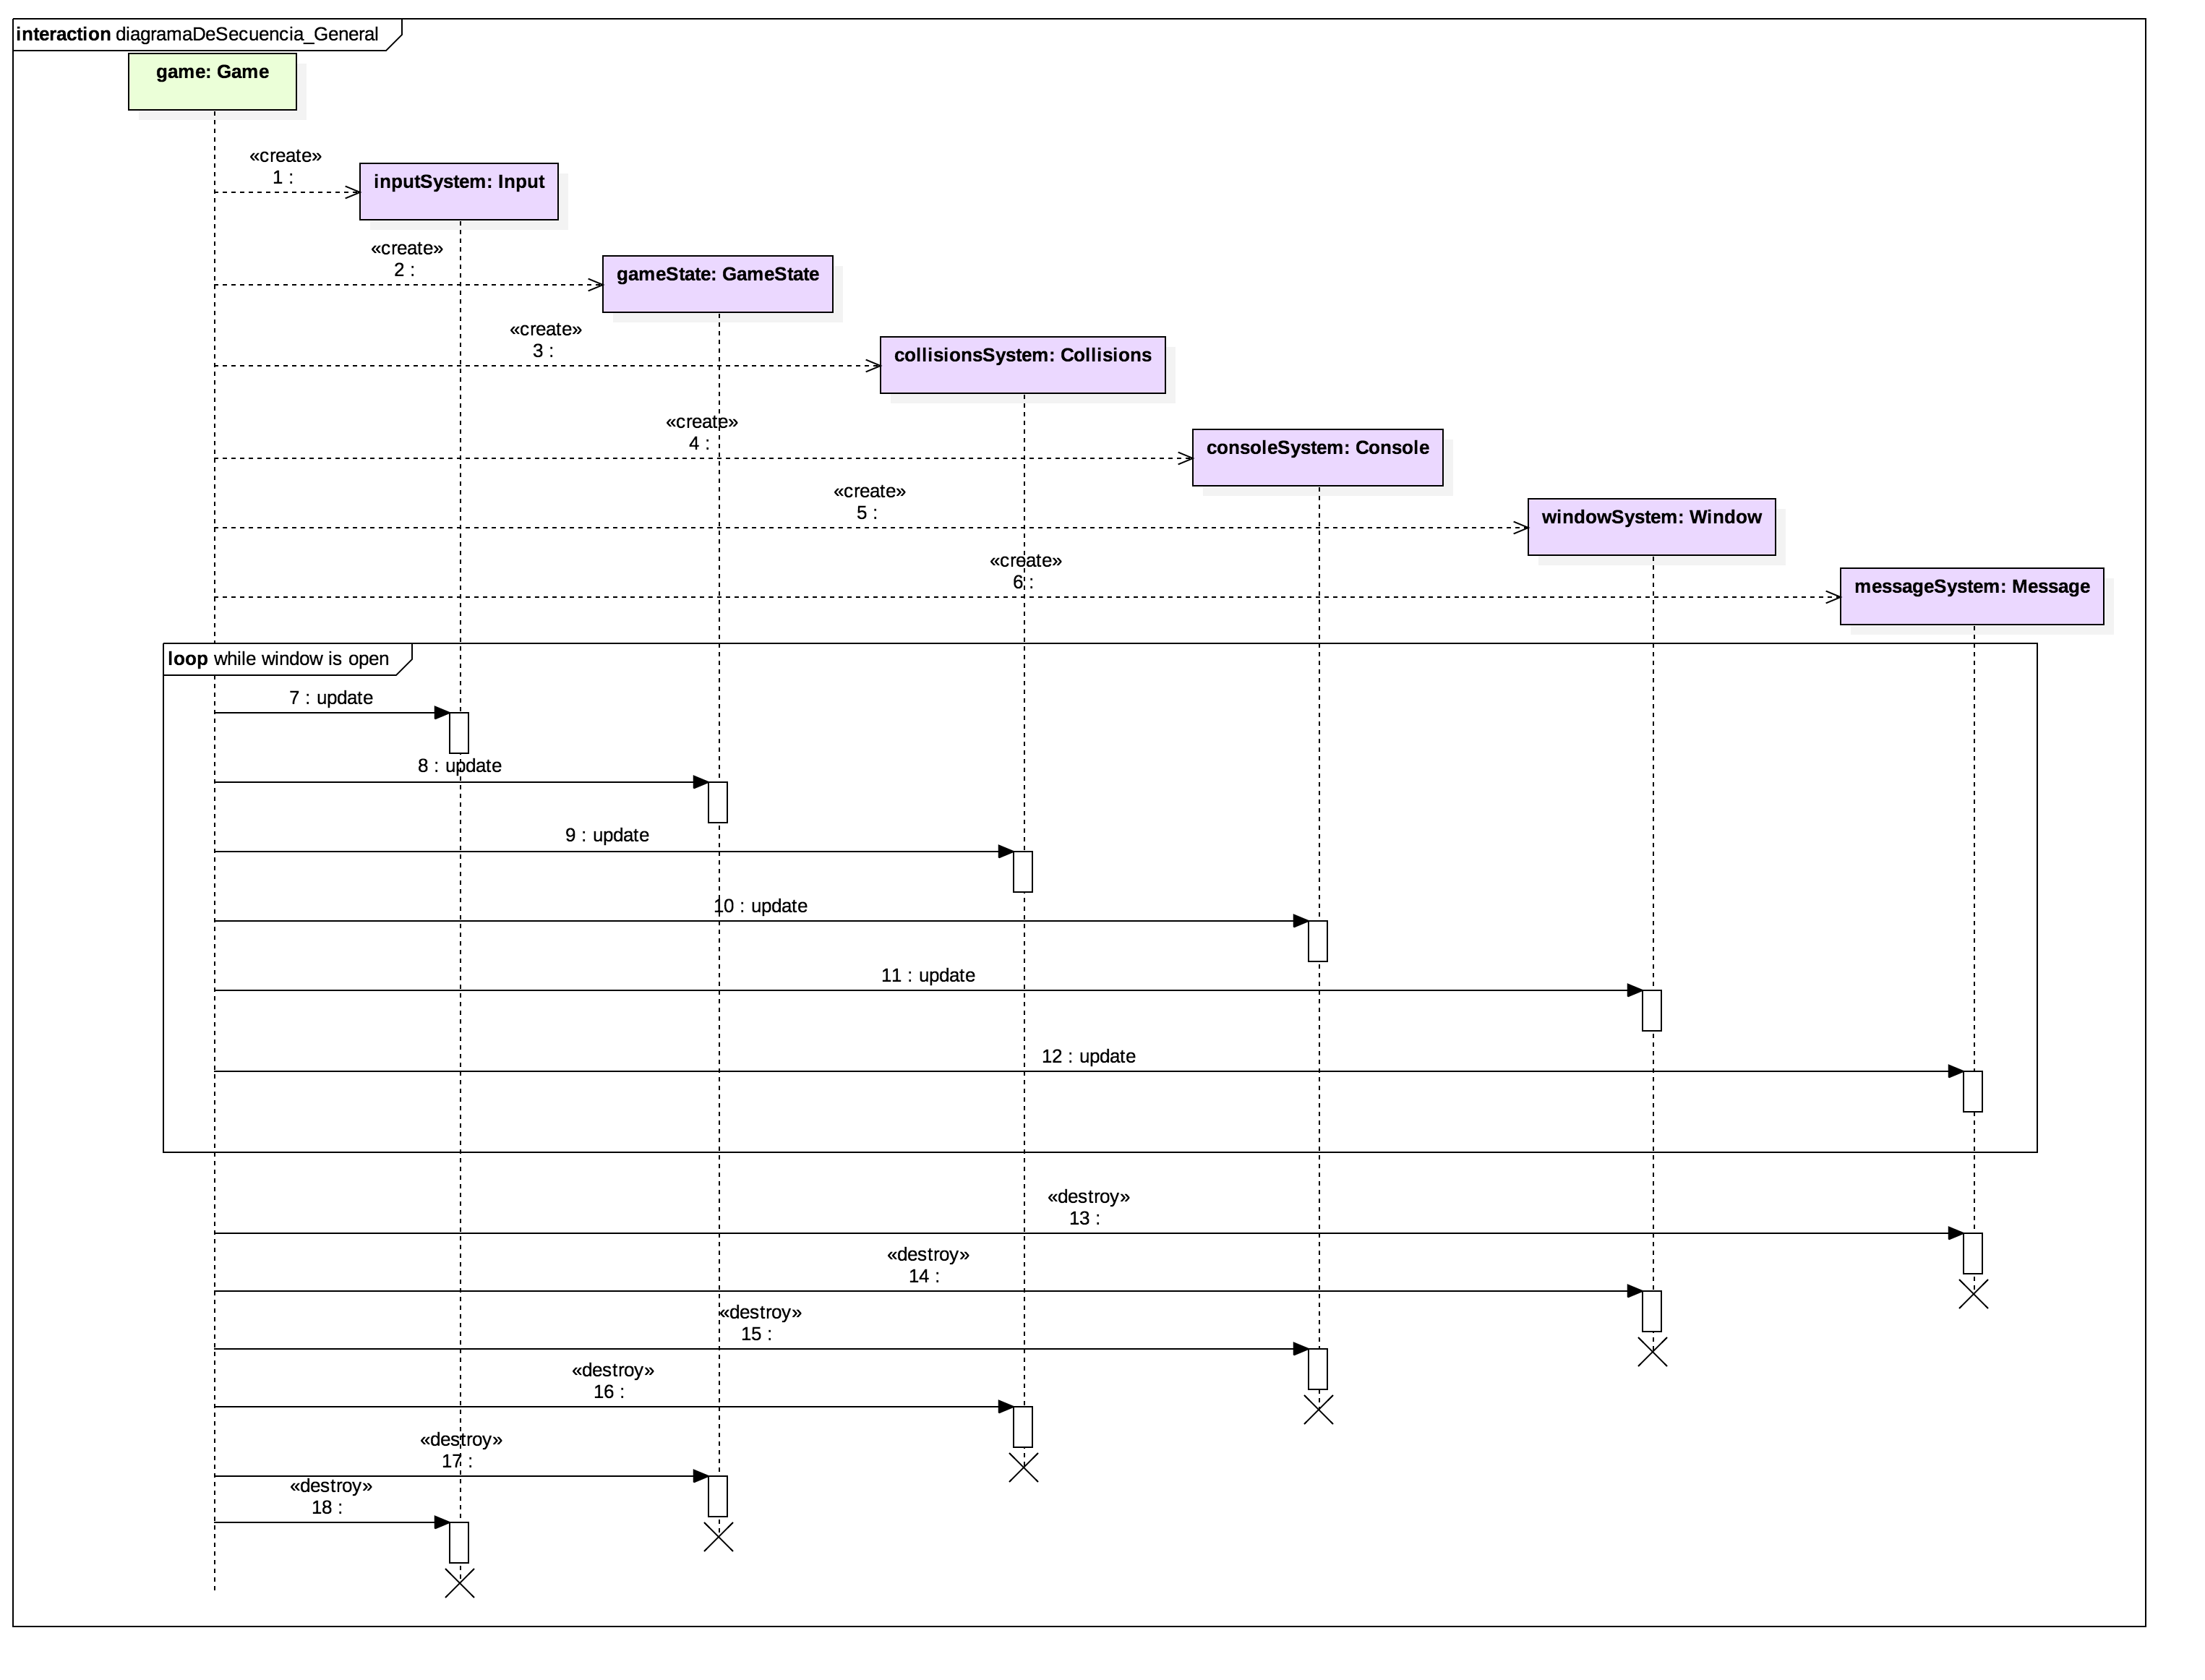
\includegraphics[width=19cm]{otros/UML/png/alld/png/CasosDeUso__General__Collaboration1__Interaction1__diagramaDeSecuencia_General_15.png}}
	\caption{Diagrama de secuencia general de la aplicación}
	\label{sec:general}
\end{figure}

\begin{figure}
	\centerline{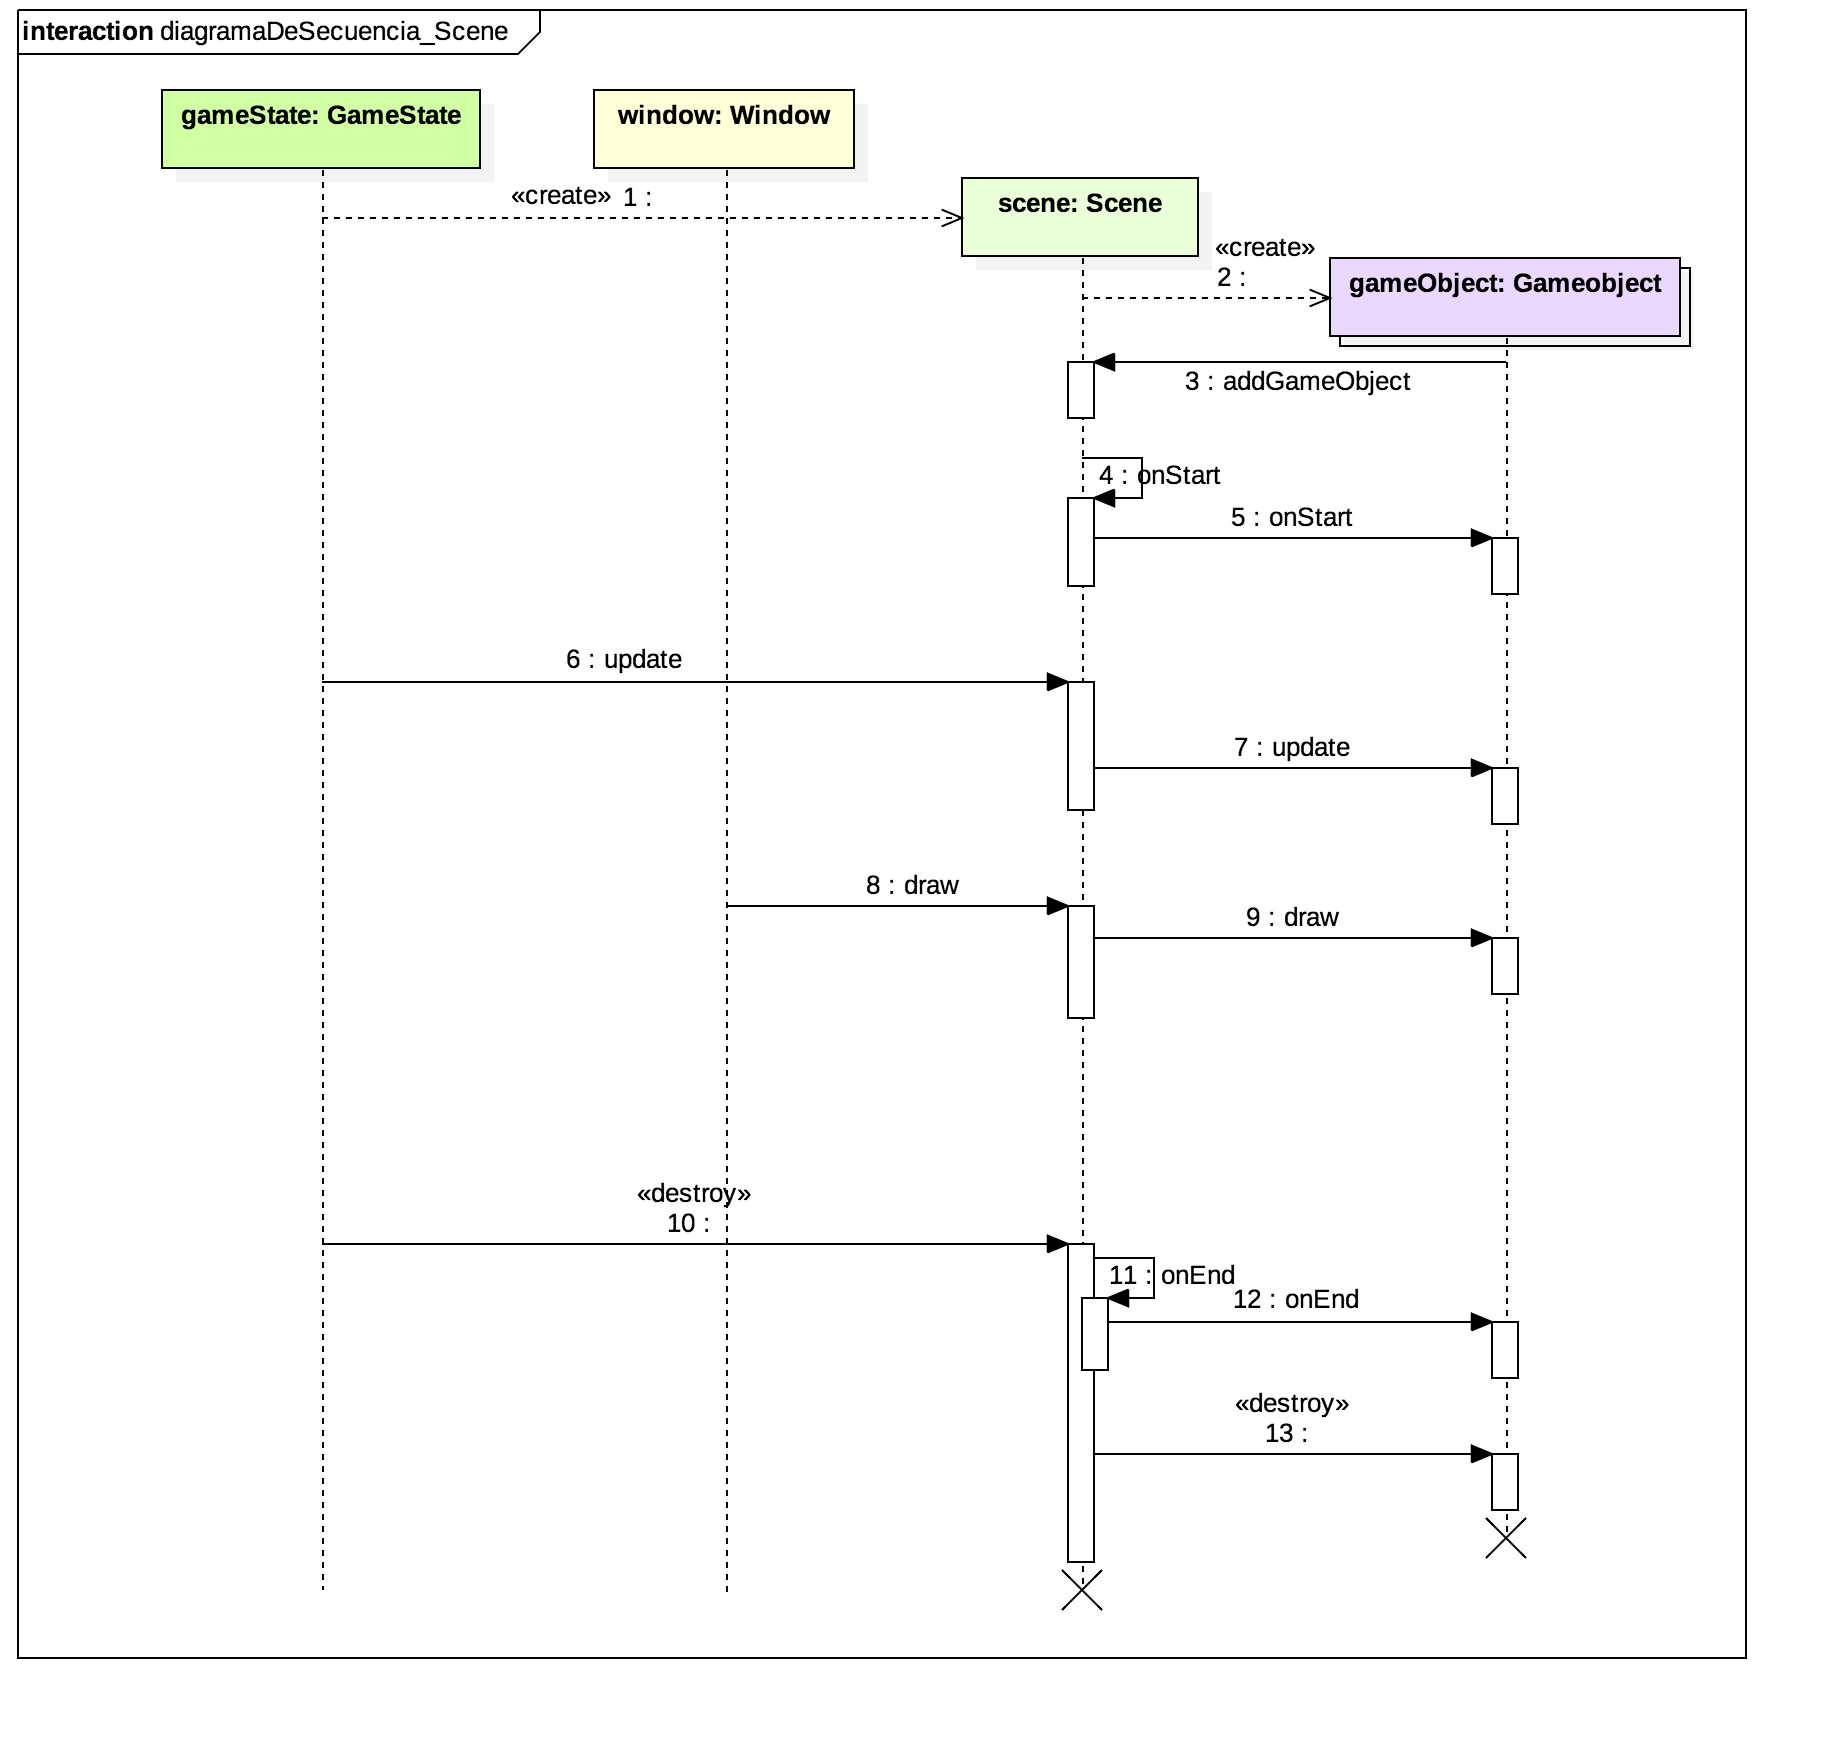
\includegraphics[width=15cm]{otros/UML/png/alld/png/CasosDeUso__General__Collaboration2__Interaction1__diagramaDeSecuencia_Scene_16.png}}
	\caption{Diagrama de secuencia genérico de una escena}
	\label{sec:scene}
\end{figure}

\begin{landscape}
\begin{figure}
	\centerline{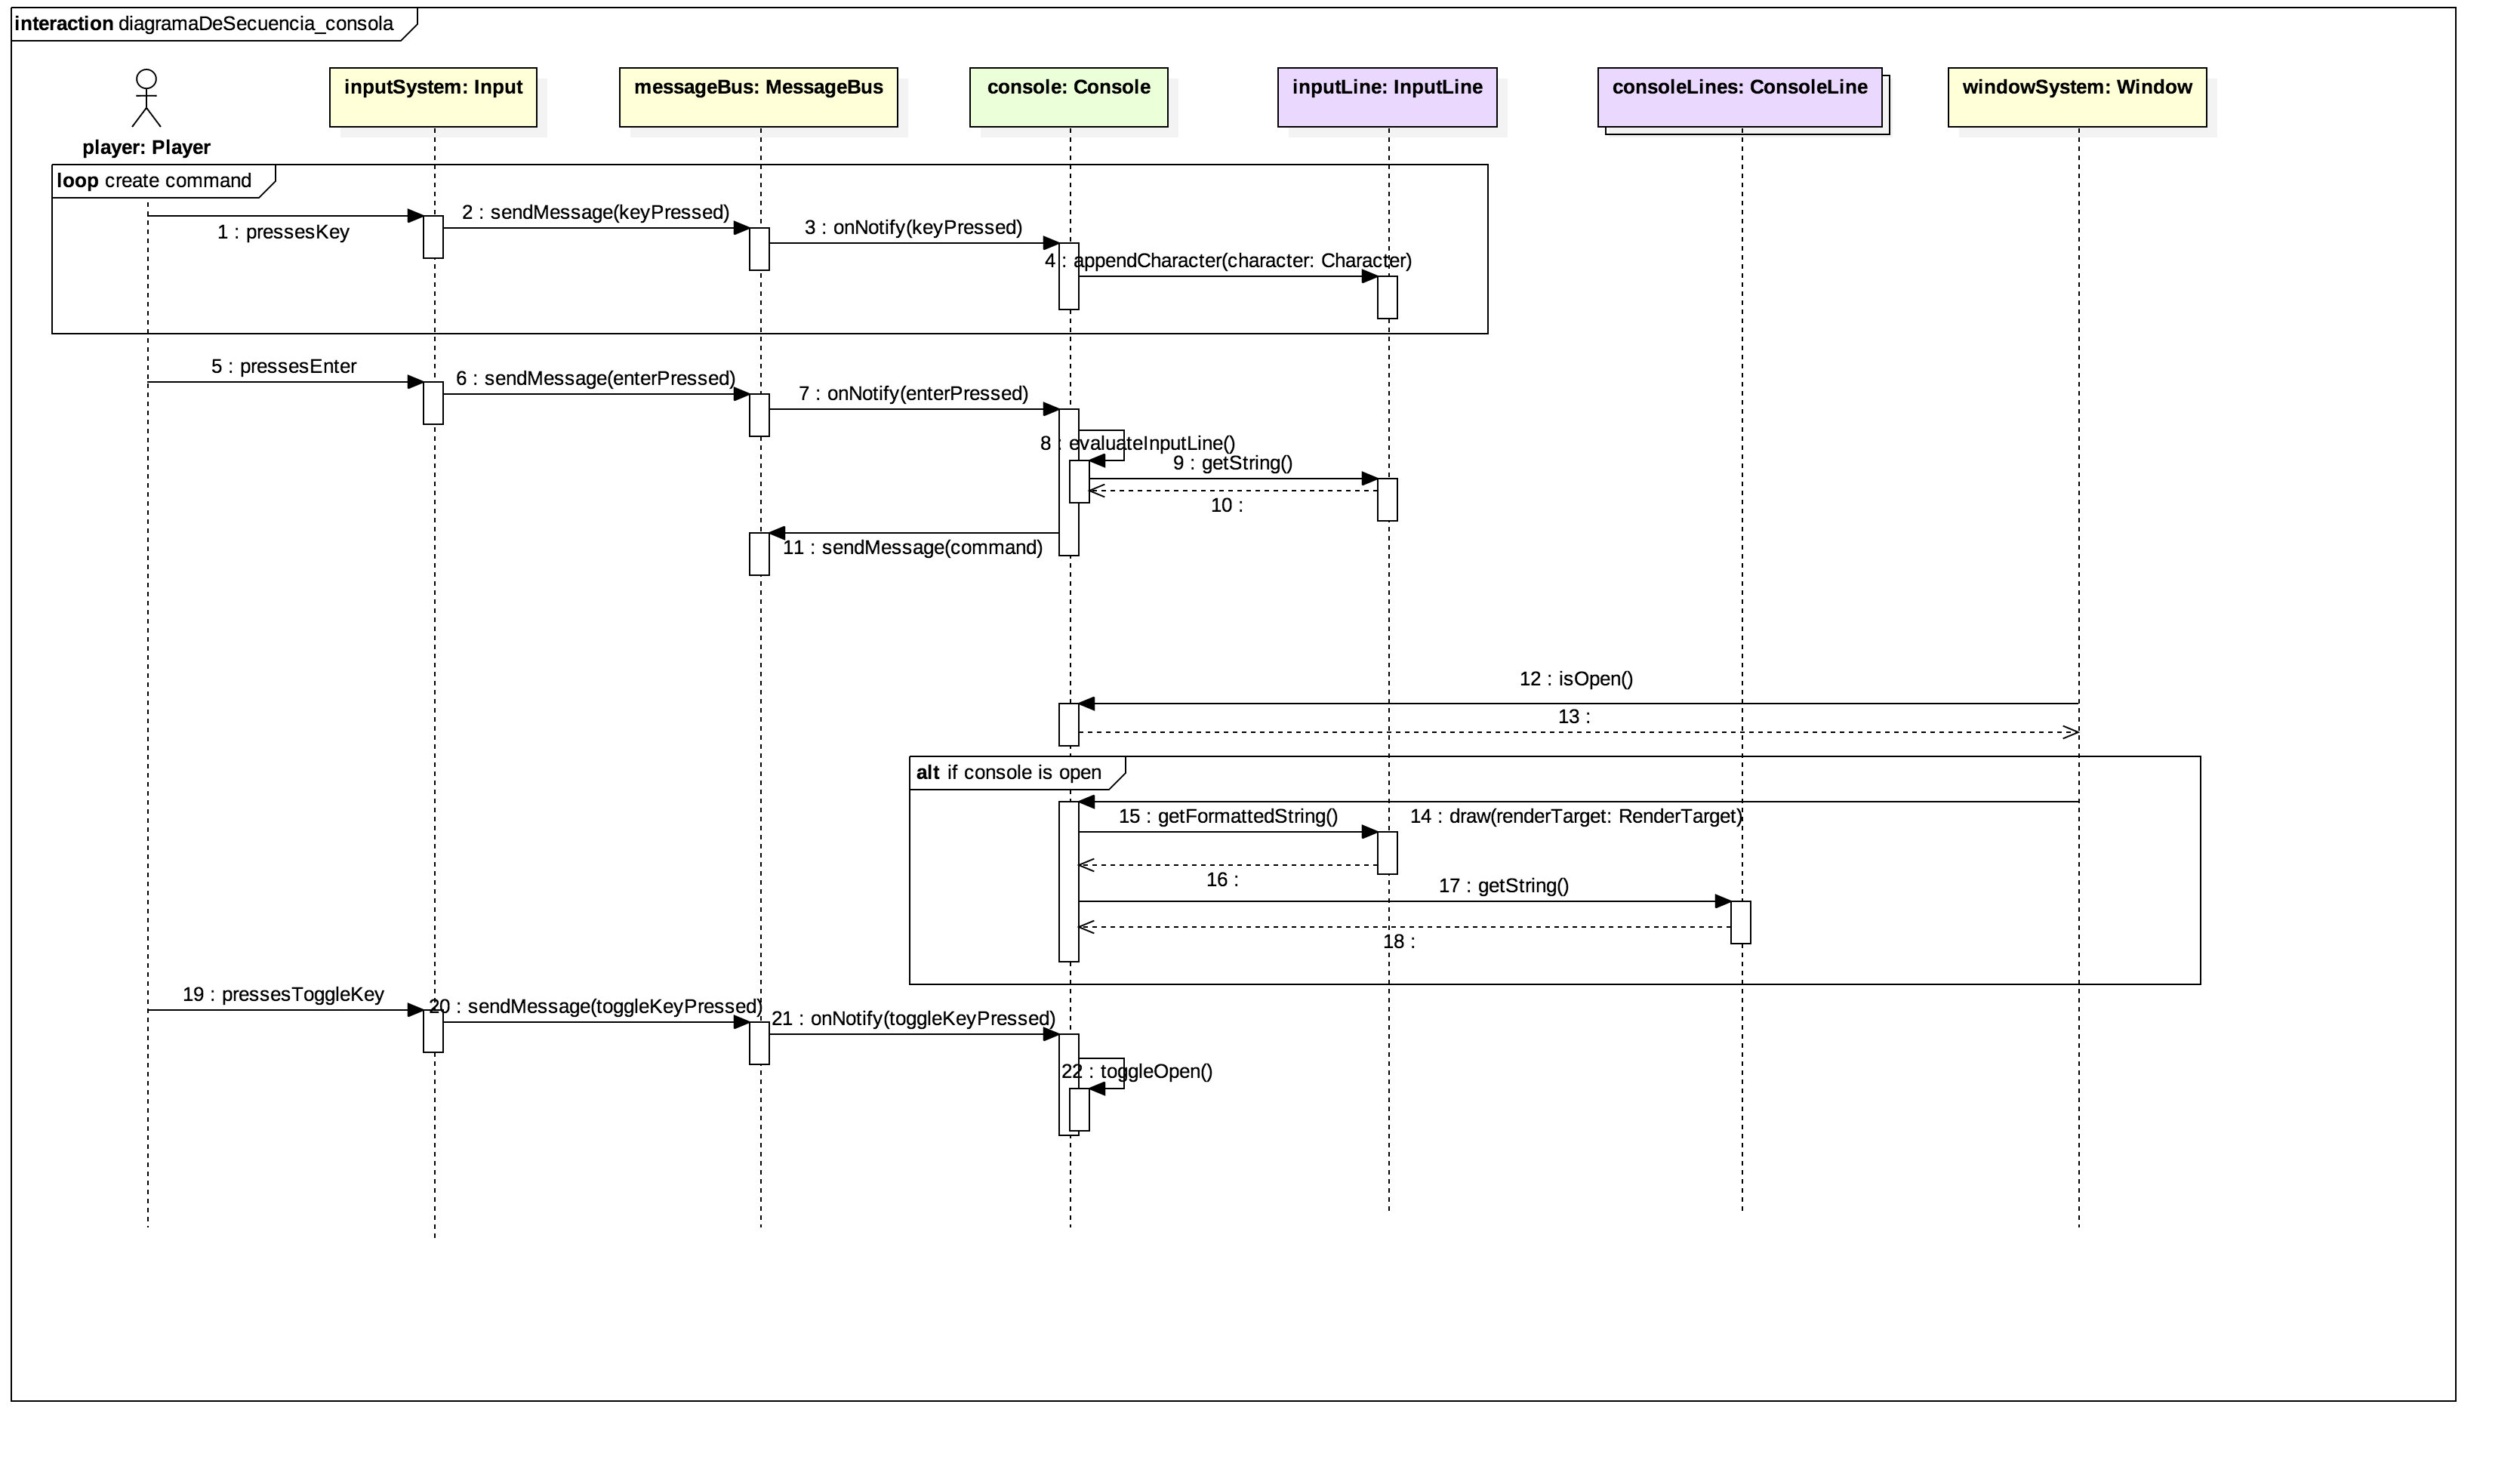
\includegraphics[width=20cm]{otros/UML/png/alld/png/CasosDeUso__Especifico__Collaboration4__Interaction1__diagramaDeSecuencia_consola_20.png}}
	\caption{Diagrama de secuencia de la consola}
	\label{sec:console}
\end{figure}
\end{landscape}

\begin{landscape}
\begin{figure}
	\centerline{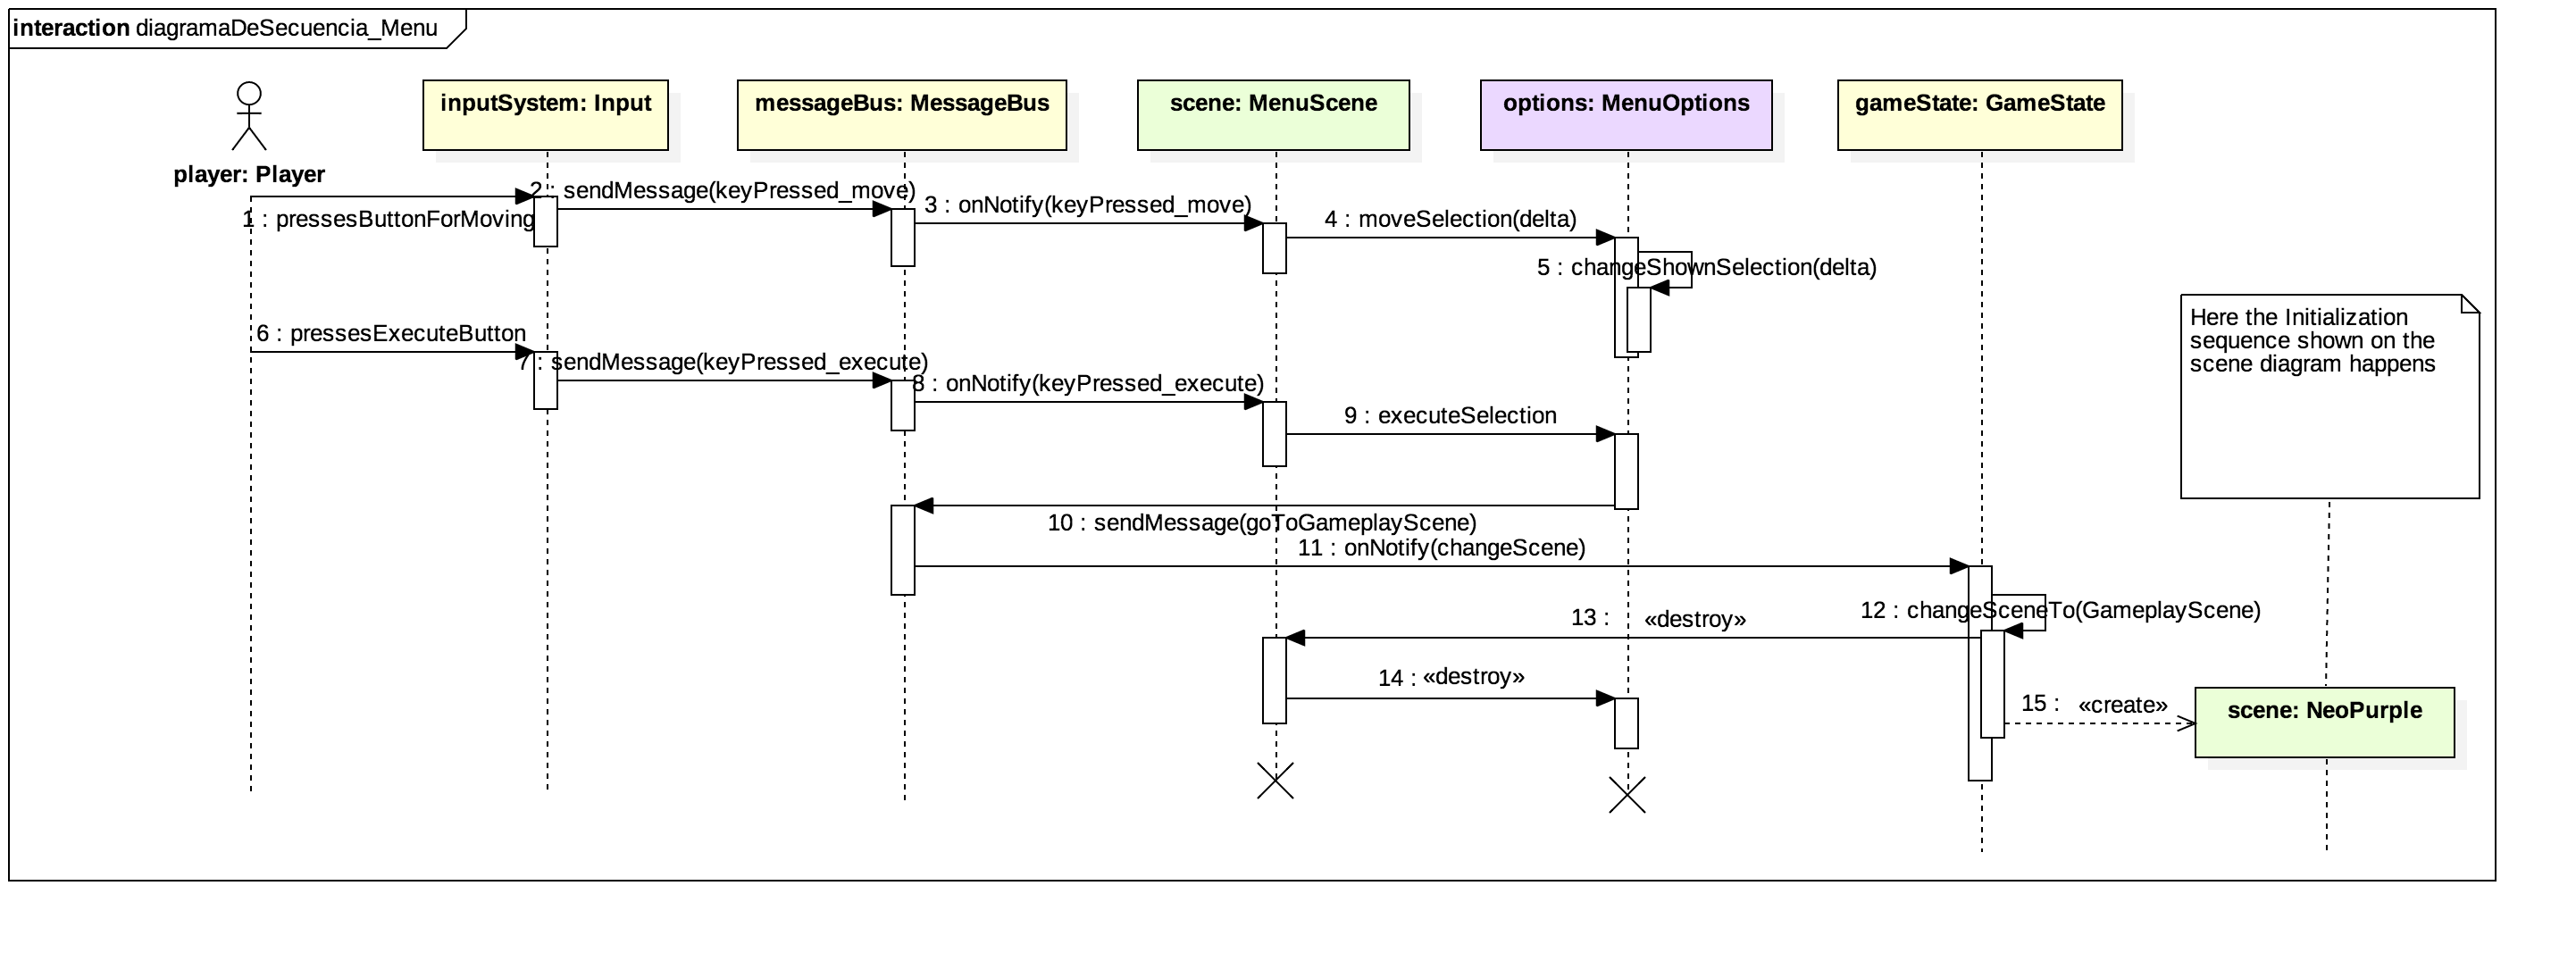
\includegraphics[width=20cm]{otros/UML/png/alld/png/CasosDeUso__Especifico__Collaboration1__Interaction1__diagramaDeSecuencia_Menu_17.png}}
	\caption{Diagrama de secuencia de la escena del menú}
	\label{sec:menu}
\end{figure}
\end{landscape}

\begin{figure}
	\centerline{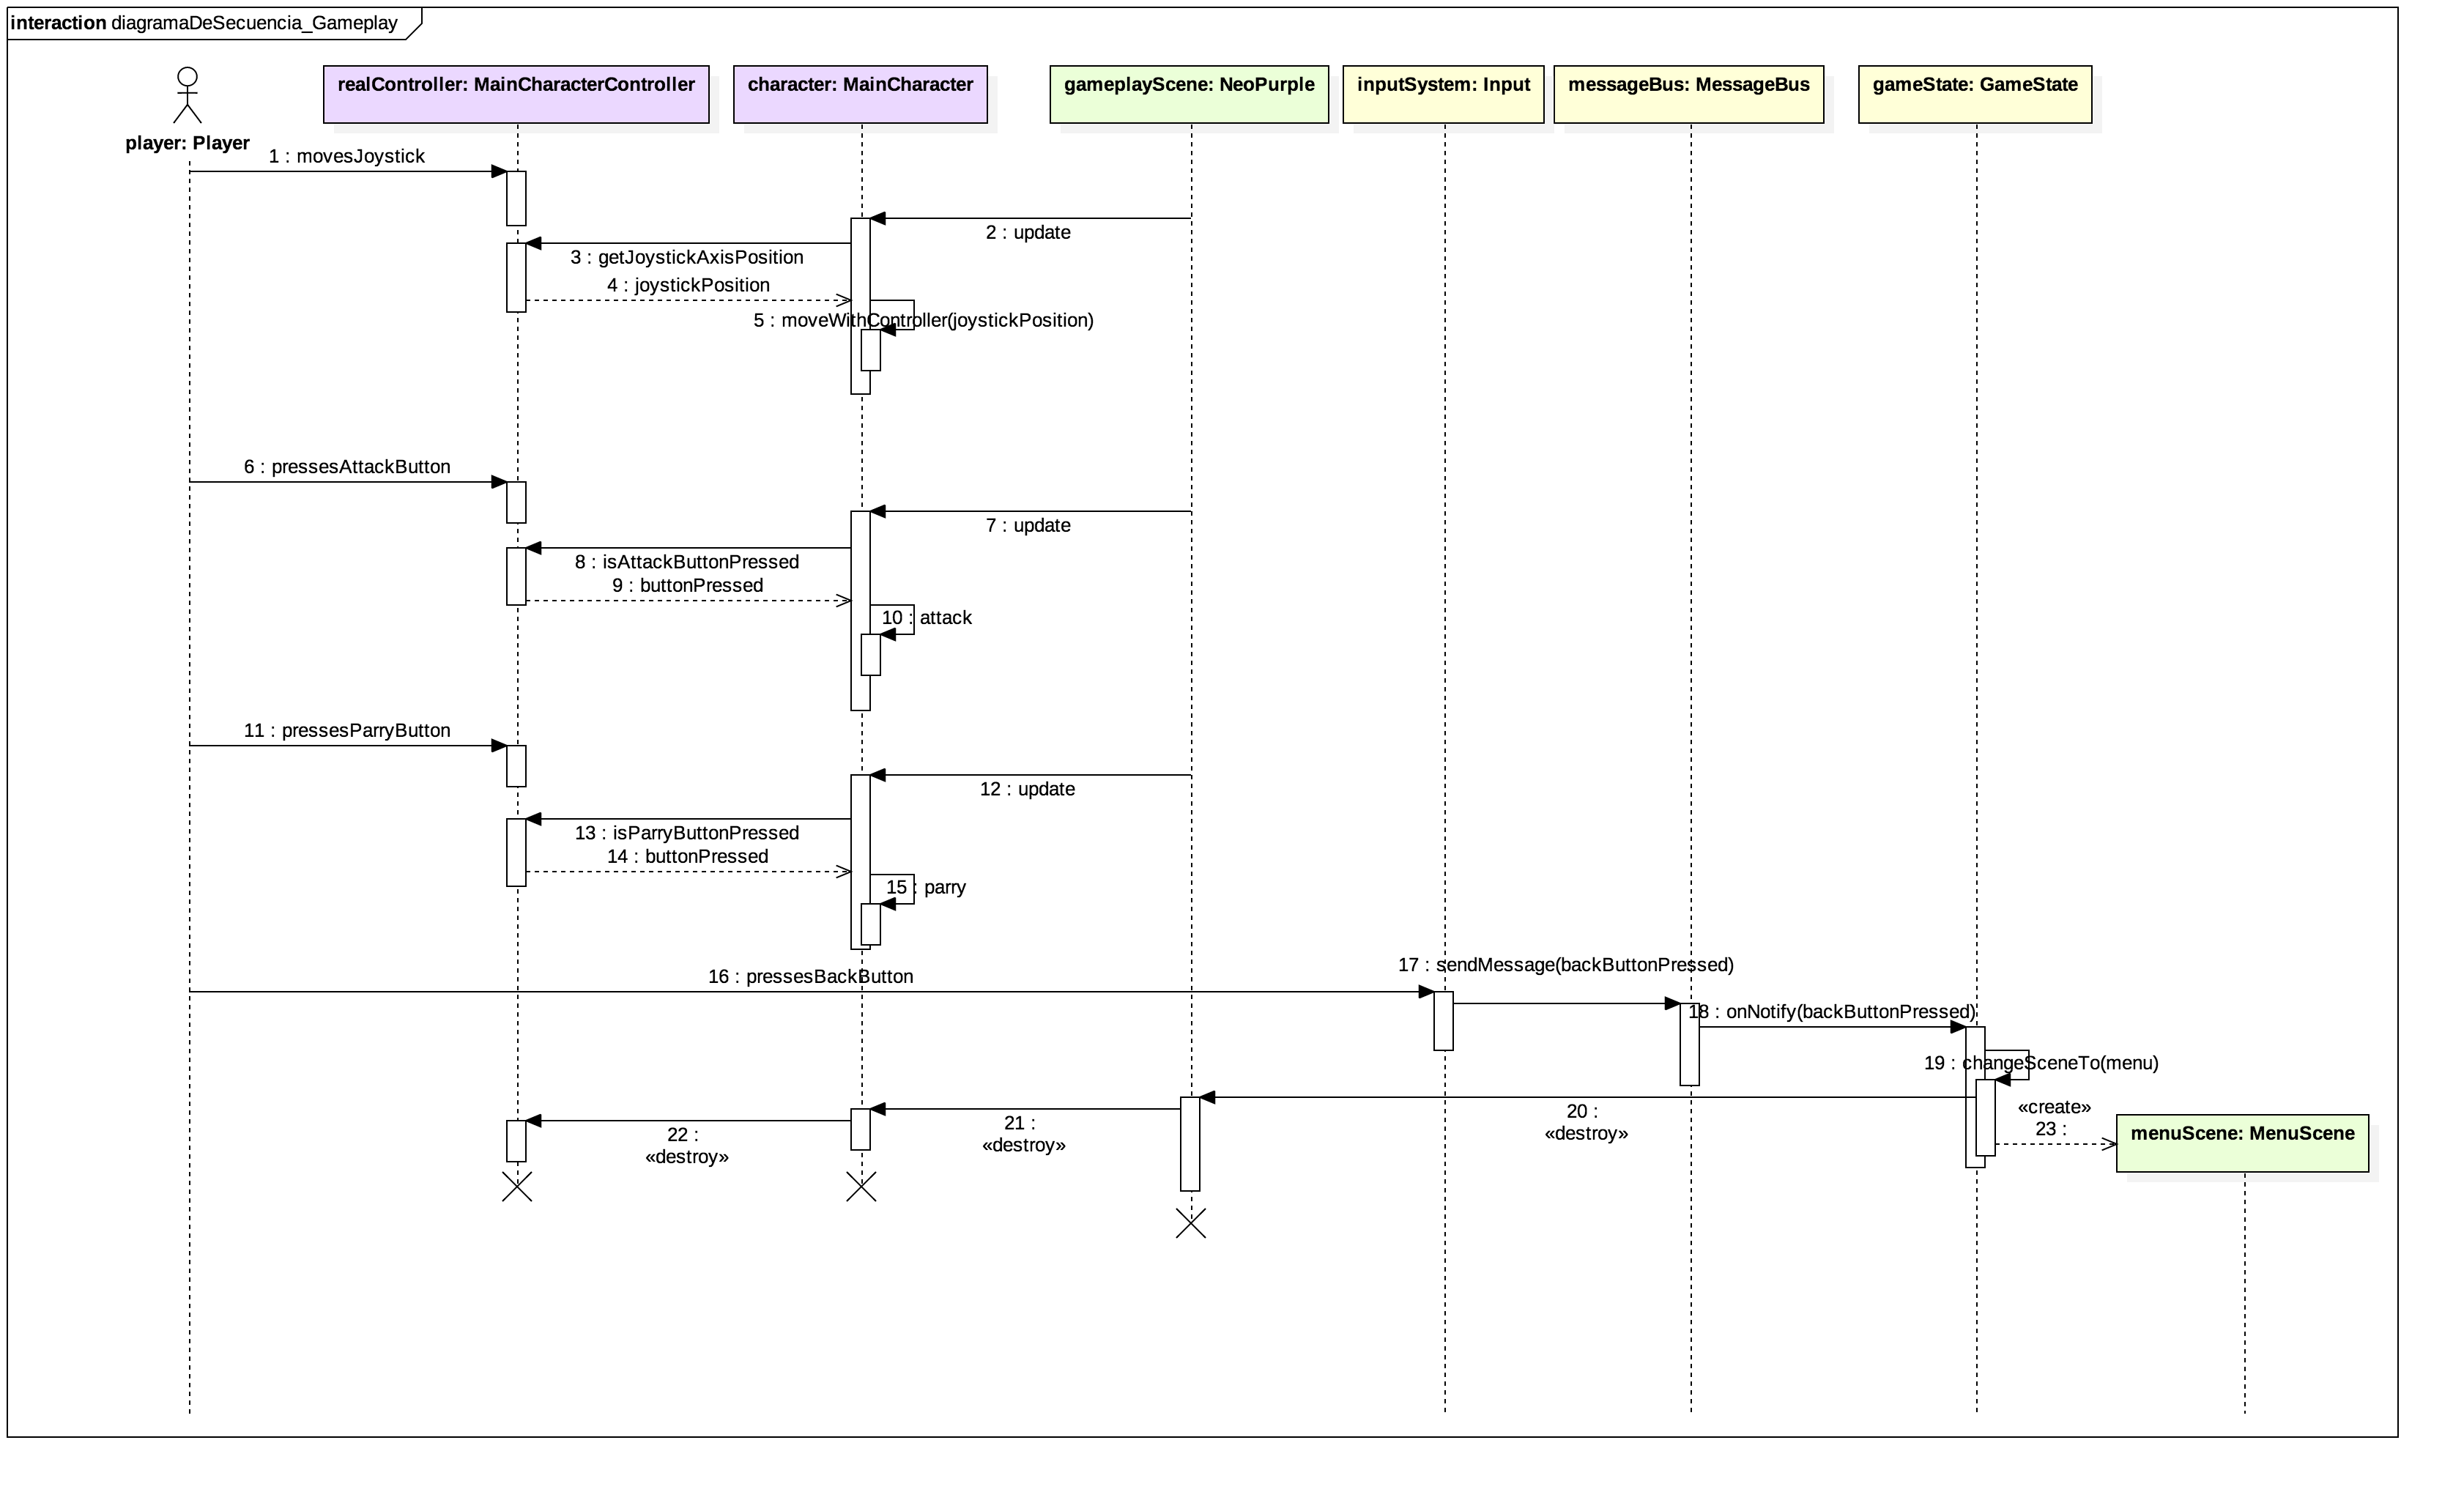
\includegraphics[width=19cm]{otros/UML/png/alld/png/CasosDeUso__Especifico__Collaboration2__Interaction1__diagramaDeSecuencia_Gameplay_18.png}}
	\caption{Diagrama de secuencia de la escena del \textit{gameplay}}
	\label{sec:gameplay}
\end{figure}

\begin{figure}
	\centerline{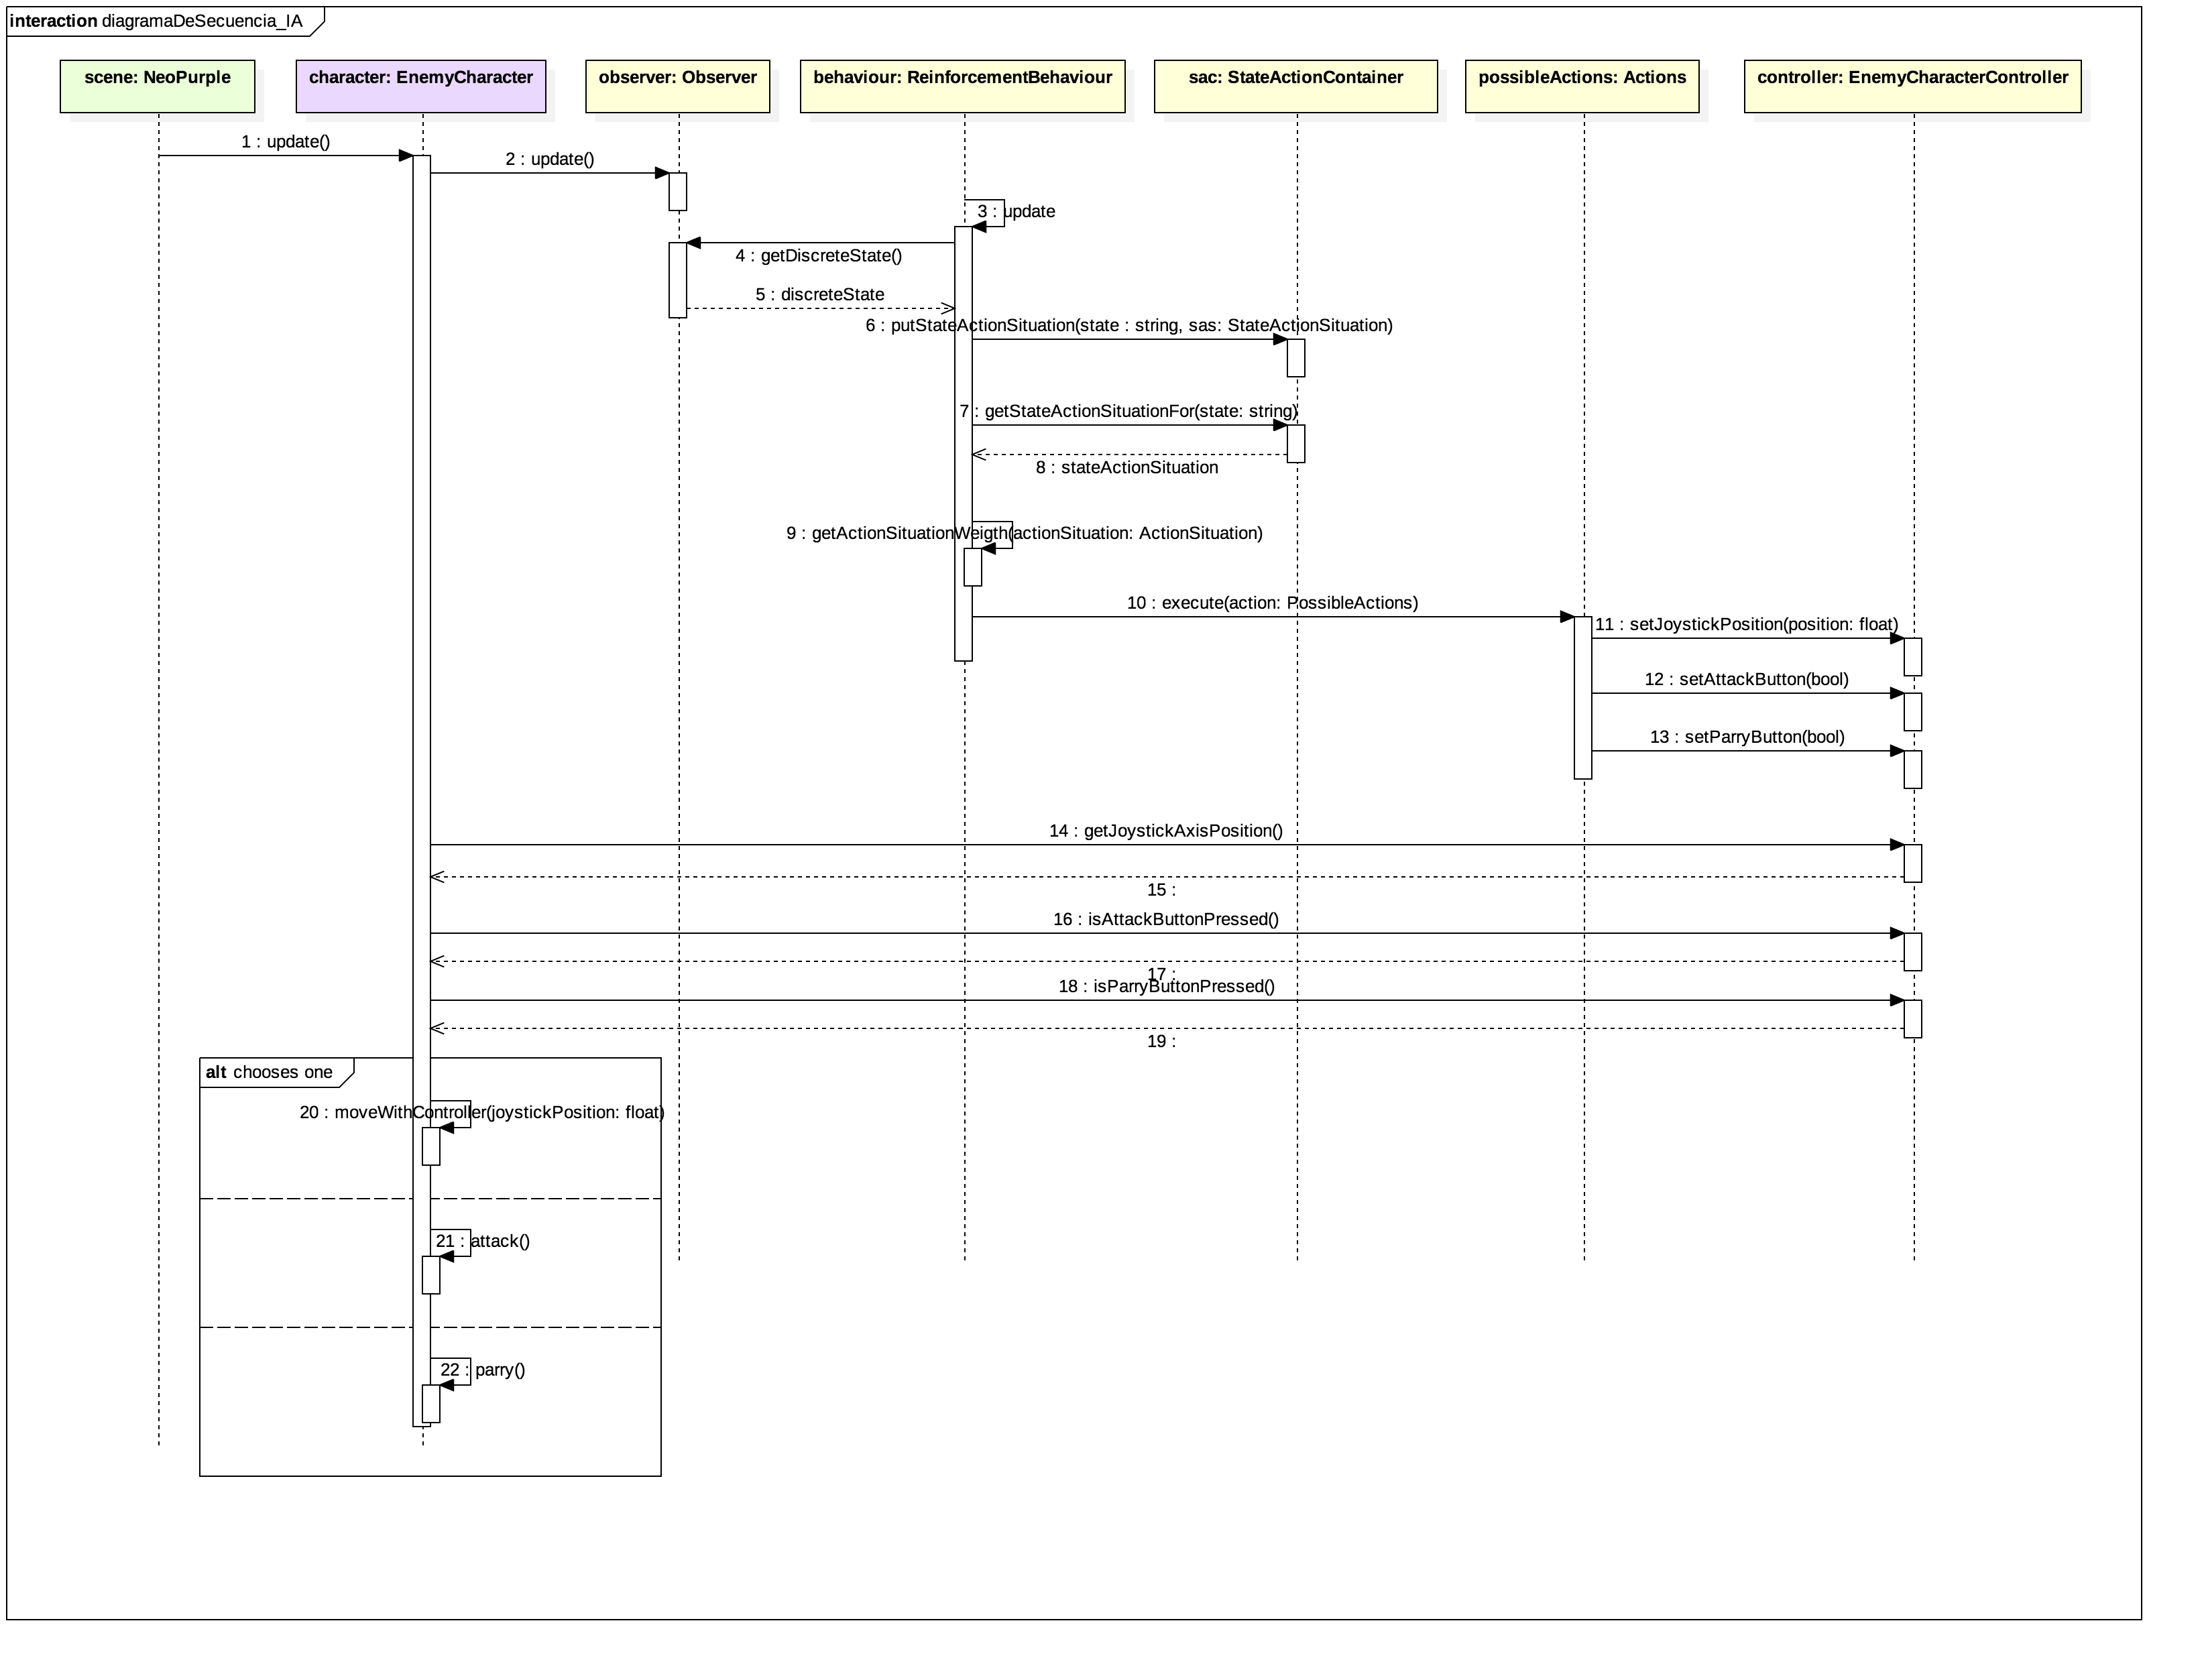
\includegraphics[width=19cm]{otros/UML/png/alld/png/CasosDeUso__Especifico__Collaboration3__Interaction1__diagramaDeSecuencia_IA_19.png}}
	\caption{Diagrama de secuencia del agente}
	\label{sec:agent}
\end{figure}

